%%TODO
%%% The time sync can not be done within the container, so the host must be sinkec before that.

\documentclass[twoside,english,brazilian]{UNISINOSartigo}
\usepackage[utf8]{inputenc} % charset do texto (utf8, latin1, etc.)
\usepackage[T1]{fontenc} % encoding da fonte (afeta a sep. de sílabas)
\usepackage{graphicx} % comandos para gráficos e inclusão de figuras
\usepackage{bibentry} % para inserir refs. bib. no meio do texto
\usepackage{verbatim}
\usepackage{tabularx}
\usepackage[table,xcdraw]{xcolor}
\usepackage[font=scriptsize]{subfig}

%=======================================================================
\unisinosbst
%=======================================================================
% Dados gerais sobre o trabalho.
%=======================================================================
%\title{Análise Comparativa entre contêineres e Máquinas Virtuais para Execução de Aplicações de Alto Desempenho na Nuvem com Elasticidade}
\title{DoCB: Um Benchmark para Avaliar as Estratégias de Contêiner e Máquina Virtual na Execução de Aplicações em Nuvem com Elasticidade}
\author{Douglas Brauner}
\authorinfo{Aluno do curso de Ciência da Computação. Email: dbrauner@edu.unisinos.br}
\degree{Bacharel em Ciência da Computação}
\course{Curso de Ciência da Computação}
%\subtitulo{sub}
\address{São Leopoldo}
\date{2017}
\advisor[Prof.Dr.]{Rodrigo da Rosa Righi}

\advisorinfo{Orientador, professor da Unisinos, pós-doutor pelo Korean Advanced Institute of Science and Technology (2013), doutor em Ciência da Computação pela Universidade Federal do Rio Grande do Sul e pela Tecnische Universitaet Berlin (2009), Mestre em Ciência da Computação pela Universidade Federal do Rio Grande do Sul (2005).  Email: rrrighi@unisinos.br}

%=======================================================================
% Início do documento.
%=======================================================================
\begin{document}

\maketitle

%=======================================================================
% Dedicatória (opcional).
%
% O texto é normalmente colocado na parte de baixo da página, alinhado
% à direita.  Mas a formatação é basicamente livre.  Só não se escreve
% a palavra 'dedicatória'.
%=======================================================================
%\begin{dedicatoria}
%Aos nossos pais.\\[4ex] % quebra a linha dando um espaçamento maior
%\begin{itshape} % faz o texto ficar em itálico
%If I have seen farther than others,\\
%it is because I stood on the shoulders of giants.\\
%\end{itshape}
%--- \textsc{Sir Isaac Newton} % \textsc é o "small caps"
%\end{dedicatoria}

%=======================================================================
% Agradecimentos (opcional).
%=======================================================================
%\begin{agradecimentos}
%Obrigado!
%\end{agradecimentos}

%=======================================================================
% Epígrafe (opcional).
%
% ``[...] o autor apresenta uma citação, seguida de indicação de autoria,
% relacionada com a matéria tratada no corpo do trabalho. Podem, também,
% constar epígrafes nas folhas de aberturas das seções primárias.''
%=======================================================================
%\begin{epigrafe}
%``\textit{Ninguém abre um livro sem que aprenda alguma coisa}''.\\
%(Anônimo)
%\end{epigrafe}

\begin{abstract}Uma das características mais importantes da computação em nuvem é a elasticidade de recursos, capacidade na qual o ambiente computacional pode aumentar ou diminuir os recursos demandados pelo usuário. Em ambientes de processamento de alto desempenho (PAD), as aplicações são encapsuladas em máquinas virtuais para garantir isolamento e permitir migração e replicação. Hoje em dia, além de máquinas virtuais, vem crescendo a adoção de Contêineres Docker, como uma alternativa à virtualização baseadas em hipervisor, compostos de imagens leves e virtualizadas no nível de sistema operacional (SO). Porém, por serem parte de uma tecnologia emergente, as aplicações PAD ainda utilizam o método de virtualização tradicional. Os estudos na literatura não oferecem uma comparação das tecnologias voltada para elasticidade em PAD.

Nesse contexto, este trabalho apresenta o DoCB (Docker Containers Benchmark), um benchmark de avaliação entre contêineres e máquinas virtuais, utilizando cada estratégia para a execução de aplicações paralelas e distribuídas em uma nuvem. O benchmark ainda mostra uma comparação de elasticidade e o impacto na execução em paralelo. Uma ferramenta desenvolvida no grupo de pesquisa, chamada AutoElastic, é utilizada para fazer o gerenciamento das execuções com contêineres e máquinas virtuais na nuvem, os dados gerados pelo AutoElastic são utilizados para compor e comparar os resultados de ambas tecnologias. Nos testes com uma aplicação de carga ascendente, a utilização de contêineres para virtualização apresentou um desempenho expressivamente maior, com um ganho de 20\% no tempo de execução e 60\% no custo (tempo x recursos) de processamento.
\palavraschave{Computação em Nuvem.  Elasticidade.  AutoElastic.  Contêiner.  Docker}
\end{abstract}

%=======================================================================
% Lista de Abreviaturas (opcional).
%
% Deve ser passada como parâmetro a maior das abreviaturas utilizadas.
%=======================================================================
%\begin{listadeabreviaturas}{seg., segs.}
%\item[ampl.] ampliado, -a
%\item[atual.] atualizado, -a
%\item[coord.] coordenador
%\item[N.~T.] Novo Testamento
%\item[seg., segs.] seguinte, -s
%\end{listadeabreviaturas}

%=======================================================================
% Lista de Siglas (opcional).
%
% Deve ser passada como parâmetro a maior das siglas utilizadas.
%=======================================================================
%\begin{listadesiglas}{FAPERGS}
%\item[ABNT] Associação Brasileira de Normas Técnicas
%\item[CAPES] Coordenação de Aperfeiçoamento de Pessoal de Nível Superior
%\item[FAPERGS] Fundação de Amparo à Pesquisa do Estado do Rio Grande do Sul
%\end{listadesiglas}

%=======================================================================
% Lista de Símbolos (opcional).
%
% Deve ser passado o maior (mais largo) dos símbolos utilizados.
%=======================================================================
%\begin{listadesimbolos}{Ca}
%\item[\textsuperscript{o}C] Graus Celsius
%\item[Al] Alumínio
%\item[Ca] Cálcio
%\end{listadesimbolos}

%=======================================================================
% Sumário
%=======================================================================
%\tableofcontents

%=======================================================================
% Introdução
%=======================================================================
\section{Introdução}

Uma das características mais importantes da computação em nuvem é a elasticidade de recursos \cite{Mell2012,Mauch20131408}. Ou seja, a capacidade do ambiente computacional aumentar ou diminuir os recursos demandados pelo usuário. Como recursos, podemos entender tudo aquilo que representa poder computacional, como CPU, memória, rede e largura de banda \cite{Kominos2017}. Uma das técnicas para se otimizar o desempenho de aplicações elásticas é a alocação dinâmica de recursos, o que permite o provisionamento de recursos quando a aplicação está necessitando, além da liberação de recursos adicionais, quando esta mesma está operando de forma moderada. A estratégia de elasticidade irá depender do objetivo do usuário, que por exemplo, em um cenário de aplicações de Processamento de Alto Desempenho (PAD), ou \textit{High Performance Computing} (HPC), pode requisitar um aumento de poder computacional para executar uma determinada tarefa em um tempo menor. Por outro lado, se a execução não escala de forma linear e a aplicação não requer um tempo curto de processamento, a quantidade recursos pode ser reduzida, o que resultaria em um valor menor de \textit{recursos x horas} para este caso, já que a questão é a economia de recursos.

O estado-da-arte atual mostra que uma das abordagens mais comuns de elasticidade é a replicação de máquinas virtuais, quando um determinado \textit{threshold} é atingido, uma nova instância é requisitada e fornecida pelo gerenciador \cite{7090978,7185168,6217477}. Dessa forma, ambientes de PAD se beneficiam de utilização de tecnologias de virtualização para fornecer ambientes customizados para as necessidades e compartilhamento de recursos. Entretanto, aplicações de alto desempenho somente serão capazes de se beneficiar da utilização de ambientes virtualizados se não houver um \textit{overhead} substancial de desempenho: tanto no mapeamento de funções virtualizadas pelo hipervisor, quanto pelo tempo de entrega (boot) de uma máquina virtual (VM) \cite{Xavier2013}. No geral, estudos realizados mostram que os métodos tradicionais de virtualização, como Xen, VMWare e KVM possuem um overhead significativo de desempenho para alguns casos, o que dificulta a sua utilização em todas as aplicações PAD \cite{Zheng2017}. 

Algumas implementações recentes de virtualização baseada em contêineres, como Linux-Vserver, OpenVZ e Linux contêineres (LXC) oferecem uma camada leve de virtualização, com a promessa de desempenho muito próximo ao nativo, devido à sua arquitetura e virtualização no nível de sistema operacional (SO) \cite{Bernstein2014}. Ao contrário de VMs, contêineres também oferece solução sem isolamento, onde contêineres num mesmo nó concorrem de igual para igual pela totalidade dos recursos da CPU, o que pode ser vantajoso, caso eles realizem tarefas de processamento intenso. Desta forma, podemos identificar 3 modalidades para estas duas técnicas de virtualização: máquina virtual com limite de CPU (Rígido), contêiner com limite de CPU (Rígido) e contêiner sem limite de CPU (Flexível). Todavia, não há trabalhos na literatura que explorem uma análise comparativa entre as 2 técnicas e 3 modalidades no contexto de PAD, tampouco no que tange o numero de unidades executadoras (VMs ou contêineres) por nó na variação da carga em tempo de execução.

\begin{comment}
Os trabalhos vistos na literatura, apesar de mostrar um comparativo de recursos virtualizados com contêineres e VMs, não apresentam uma avaliação de contêineres para cenários de PAD, onde a elasticidade deve ser executada. Assim, não é possível identificar qual tecnologia é a mais indicada para a situação, além disto, a granularidade de instâncias e o custo computacional também não são explorados.
\end{comment}
Neste contexto, o presente artigo propõe o Docker Containers Benchmark (DoCB), uma avaliação de contêineres e máquinas virtuais, utilizando estratégias de cada alternativa, para a execução de aplicações paralelas e distribuídas em uma nuvem. O benchmark ainda mostra uma comparação de desempenho ao variar o número de unidades de processamento virtualizadas (contêiner ou VM), na execução em de uma aplicação em paralelo. O estudo mostra que contêineres conseguem tirar muito mais proveito da elasticidade na nuvem, agilizando a entrega de recursos quando for solicitado, o benchmark ainda mostra a maleabilidade de CPU na utilização vários contêineres em paralelo em uma mesma máquina, ou seja, a diferença que se obtêm ao não definir limite de CPU por contêiner. O DoCB foi avaliado com a adaptação de um modelo chamado AutoElastic \citetexto{7090978}, o qual foi utilizado para fazer o gerenciamento das execuções com contêineres e máquinas virtuais na nuvem, os dados gerados pelo AutoElastic são utilizados para compor e comparar os resultados de ambas tecnologias. 

Este trabalho foi organizado em 8 seções. Nesta seção falamos do tema do trabalho e introduzimos o assunto abordado. Na sequência, iremos apresentar uma revisão dos conceitos por trás das tecnologias utilizadas e revisaremos o estado-da-arte. Na seção \ref{related} é feito um estudo de trabalhos relacionados ao tema deste artigo. Na seção \ref{model} será apresentado o benchmark criado, com detalhes da metodologia empregada na execução. Teremos então, na seção \ref{avaliacao} uma análise dos resultados obtidos utilizando os critérios definidos. Finalmente, a seção \ref{conclusion} é destinada às considerações finais do trabalho, bem como oportunidades de trabalhos futuros.

\section{Fundamentação Teórica}
\label{fundamentacao}
\begin{comment}

\section{Questão de Pesquisa}

Aplicações HPC exigem que o ambiente em que estão sendo executadas, normalmente um cluster privado com recursos limitados, forneça a capacidade para executar os processos com máxima eficiência. Porém, estes ambientes encaram um problema de balanço entre alocação eficiente de recursos e o tempo mínimo de execução para aplicações HPC. Esta sobrecarga ocorre porque para cada máquina virtual (VM) criada, necessita-se a instalação de um sistema operacional convidado (\textit{Guest OS}), alocado pelo \textit{hypervisor}, esta abordagem requer recursos de memória e utiliza parte dos recursos que poderiam estar sendo utilizados pelas aplicações HPC \cite{Adufu2015}. Em consequência deste gerenciamento, a sobrecarga de uma máquina virtual pode ser um fator de grande impacto na aplicação, se não for corretamente configurado. Algumas análises de desempenho de aplicações HPC, utilizando algoritmos de \textit{benchmark}, identificaram uma sobrecarga de 17\% de utilização de CPU, quando executando uma máquina virtual, mas que após um ajuste fino, perdeu de apenas 2\% na questão de desempenho, em comparação ao processamento nativo \cite{Stenberg2016}.

Aplicações HPC iterativas são, em sua maioria e independente da aplicabilidade, algoritmos estruturados em laços iterativos (\textit{loops}), que representam um estado global consistente a cada iteração no laço \cite{Facco2016}. Para uma aplicação HPC, questões de desempenho são fundamentais, em certos casos, a diferença de alguns milissegundos é o suficiente para distinguir uma aplicação lenta de uma rápida. A ideia é que os modelos de elasticidade possam ser executados sem realizar impacto significativo na execução da aplicação, fornecendo recursos necessários da forma mais eficiente possível. Tendo em vista o \textit{overhead} que a utilização de máquinas virtuais podem acrescentar no desempenho de uma aplicação HPC iterativa, podendo também olhar para a elasticidade que contêineres oferecem, o trabalho aqui disposto busca responder a seguinte questão:

	\textit{É possível melhorar o modelo de elasticidade em nuvem para aplicações HPC iterativas, a partir da utilização de contêineres, diminuindo o tempo de provisionamento, bem como o processamento gasto com gerenciamento de recursos?} 


\section{Objetivos} 
	O objetivo geral deste trabalho é:
	\begin{itemize}
		\item Implementar um \textit{benchmark} de avaliação entre contêineres e Máquinas Virtuais para execução de aplicações HPC em nuvem com elasticidade.
	%\item Desenvolver uma melhoria para o modelo de elasticidade automática aplicações de Computação de Alto Desempenho, buscando otimizar a elasticidade e utilização de recursos, a partir da utilização de contêineres.  
	\end{itemize}
	Para atingir o objetivo acima citado, temos os seguintes objetivos secundários:
	\begin{itemize}
		\item Identificar as lacunas no estado da arte de computação em nuvem, em relação à estratégias de instanciação de recursos virtuais;		
		\item Desenvolver uma melhoria para o modelo de elasticidade automática aplicações de Computação de Alto Desempenho, buscando otimizar a elasticidade e utilização de recursos, a partir da utilização de contêineres.
		\item Desenvolver uma estratégia de comparação com o \textit{estado da arte} de elasticidade, utilizando VMs;
		\item Desenvolver uma aplicação iterativa de alto desempenho para execução e simulação em nuvem;
		\item Realizar testes em laboratório, utilizando a aplicação desenvolvida e confrontando modelo de estado da arte e modelo proposto;
		\item Desenvolver melhoria para o algoritmo de instanciação de recursos para melhor uso de contêineres.
	\end{itemize}

\section{Organização do Texto}

Esta monografia está organizada em cinco seções. Primeiramente, na seção \ref{fundamentacao}, iremos revisar questões fundamentais a respeito da área da computação em nuvem, e as definições que relevantes ao propósito deste trabalho. Uma retomada dos tópicos relacionados à virtualização faz necessária, bem como questões gerais sobre a utilização de contêineres e tecnologias disponíveis. Na seção \ref{related}, iremos avaliar trabalhos correlatos na área, e suas contribuições para modelos de elasticidade de aplicações HPC. Além disto, será feita uma análise de trabalhos que comparam diferentes modelos de virtualização e as oportunidades da utilização de contêineres. Esta avaliação tomará como objetivo traçar uma comparação das soluções propostas, suas divergências e convergências, com o intuito de identificar lacunas e oportunidades
de trabalho na literatura analisada. A seção \ref{model} trará o modelo proposto, descrevendo sua arquitetura e metodologia para avaliação. Finalmente, a conclusão será apresentada na seção \ref{conclusion}, com detalhamento das contribuições esperadas e
um cronograma para o projeto.

%=======================================================================
% Fundamentação Teórica
%=======================================================================
\end{comment}

Este capítulo irá abordar as principais definições relacionadas ao conceito de Computação em Nuvem, levando em consideração o estado atual na área. Serão apresentados também conceitos necessários ao entendimento das motivações do projeto que levaram à definição do benchmark DoCB. Primeiramente, serão apresentados os conceitos e características de Computação em Nuvem, seguido posteriormente, dos conceitos relevantes ao entendimento da tecnologia de contêineres e a ferramenta mais utilizada atualmente no mercado, o Docker. Para finalizar, será traçado um comparativo entre as alternativas de virtualização: por máquinas virtuais ou contêineres. 

\subsection{Computação em Nuvem}
\label{cloud}
Segundo a definição do National Institute of Standards and Technologies (NIST) \cite{Mell2012}, a computação em nuvem é um modelo que permite o acesso de recursos computacionais configuráveis e compartilhados, de forma conveniente, ubíqua e sob demanda, capazes de ser provisionados e entregues com baixo custo de gerenciamento e sem a intervenção de um provedor de serviços. Tais recursos podem ser: redes, servidores, serviços, armazenamento, aplicações, etc. Tais recursos são tipicamente fornecidos no modelo \textit{pay-as-you-go}, ou seja, você paga de acordo com a demanda de recursos solicitada \cite{Suleiman2012}. Sendo assim, a computação em nuvem se utiliza de mecanismos para escalar estes recursos conforme necessidade, através de algoritmos que irão trabalhar no balanceamento de carga rapidamente para diminuir o desperdício de recursos computacionais.

Na computação em nuvem, existem cinco características essenciais que ajudam a defini-la, que são a clara distinção com outros paradigma, a elasticidade rápida dos recursos, medição de serviço, serviço sob demanda, pool de recursos e o amplo acesso ao meio\cite{Moreira2010}. Em relação à elasticidade, \citetexto{Taurion2012} define que elasticidade é a capacidade do ambiente computacional da nuvem aumentar ou diminuir de forma automática os recursos computacionais demandados e provisionados para cada usuário. Diferente da escalabilidade que se diz respeito à quantidade de usuários que ela pode manter conectados ao mesmo tempo, sendo o limite de escalabilidade o ponto em que esta não pode suportar mais usuários conectados sem apresentar a mesma  eficiência \cite{Wilder12}. 

A elasticidade é a escalabilidade em duas direções: tanto cresce quanto diminui a capacidade ofertada. Os dois termos podem ser confundidos, já que dizem respeito à adaptação de recursos conforme demanda, porém a escalabilidade é relativa à capacidade manter o desempenho conforme a demanda, já a elasticidade é a capacidade de fazer os recursos se adaptem à carga, seja para aumentar ou diminuir. 
Iremos adotar a definição de \citetexto{coutinho2013elasticidade} que diz que a elasticidade é a \textit{``Capacidade de adicionar e remover recursos de forma automática de acordo com a carga de trabalho sem interrupções e utilizando os recursos de forma otimizada``.}


\begin{comment}
\section{Elasticidade vs Escalabilidade}
\label{elastic}

A escalabilidade de uma aplicação se diz respeito à quantidade de usuários que ela pode manter conectados ao mesmo tempo, sendo o limite de escalabilidade o ponto em que esta não pode suportar mais usuários conectados sem apresentar a mesma  eficiência \cite{Wilder12}. Uma aplicação pode ter a sua escalabilidade estendida através do fornecimento de recursos de \textit{hardware} adicionais, como memória, CPU, largura de banda, etc. No contexto de uma aplicação HPC, uma escalabilidade não se detêm apenas ao número de usuários suportados, mas também ao tipo de processamento que a aplicação precisa executar e que pode precisar de recursos adicionais para continuar desempenhando de forma efetiva. Dessa forma, um sistema é dito escalável quando seu desempenho não se degrada significantemente com o aumento dos usuários ou carga.
Segundo \citetexto{Taurion2012}, elasticidade é a capacidade do ambiente computacional da nuvem aumentar ou diminuir de forma automática os recursos computacionais demandados e provisionados para cada usuário. É a escalabilidade em duas direções: tanto cresce quanto diminui a capacidade ofertada. Os dois termos podem ser confundidos, já que dizem respeito à adaptação de recursos conforme demanda, porém a escalabilidade é relativa à capacidade manter o desempenho conforme a demanda, já a elasticidade é a capacidade de fazer os recursos se adaptem à carga, seja para aumentar ou diminuir. 
Iremos adotar a definição de \citetexto{coutinho2013elasticidade} que diz que a elasticidade é a ``Capacidade de adicionar e remover recursos de forma automática de acordo com a carga de trabalho sem interrupções e utilizando os recursos de forma otimizada.``.
\end{comment}

\subsection{Docker}
\label{docker}

O Docker, apesar de inicialmente utilizar o LXC como provedor de \textit{runtime}, criou uma implementação própria de ferramenta para criação de contêineres, procurando resolver algumas limitações da implementação de LXC, como segurança e simplificação, a ferramenta é atualmente a forma de gerenciar contêiner mais popular \cite{Pahl2015}. Segundo \cite{NICKOLOFF2016}, Docker pode ser descrito como um conjunto de ferramentas e serviço que facilitam a criação e manipulação de contêineres dentro de um sistema baseado em UNIX.
Alguns dos conceitos chave para compreender a tecnologia são descritos abaixo \cite{whitepaperDocker2016}:  

\begin{itemize}
	\item Contêiner: A palavra contêiner \textit{container} se refere a uma técnica de isolamento de recursos dentro de um sistema operacional baseado em UNIX, utilizando uma série de ferramentas que trabalham nativamente, mas sem a sobrecarga de rodar um \textit{kernel} separado e sem fazer simulação de hardware, através de utilização de \textit{namespaces}, e \textit{control groups} \cite{LXC2016}.
	\item Cgroups: Cgroups é uma configuração que faz parte do subsistema de \textit{kernel} de sistemas baseado em UNIX, que fornece controle sobre recursos do sistema, como CPU, memória, rede, etc  \cite{NICKOLOFF2016}.
	\item Chroot: (\textit{change root}) é um comando Linux para mudar o diretório raiz do processo corrente e seus processos aninhados para um novo diretório. Alguns contêineres utilizam este comando para isolar e compartilhar o sistema de arquivos entre os ambientes contêinerizados \cite{Dua2014}. 
\end{itemize}

\subsection{Virtualização vs Contêinerização}
\label{virtualization}
Uma camada de virtualização pode ajudar a isolar um ambiente compartilhado de computadores. Em uma Nuvem de PAD, normalmente os recursos são compartilhados entre mais usuários e isto faz com que possa ocorrer problemas nesse compartilhamento \cite{Xavier2013}. É possível utilizar uma nuvem sem virtualização, o que trará vantagens em relação ao desempenho e evita o \textit{overhead} nos recursos, porém isto também significa falta de flexibilidade, e dificuldade de utilização, pois os recursos não são compartilhados entres o nós \cite{Kominos2017}. Um hipervisor (\textit{hypervisor}), ou gerenciador de máquinas virtuais, é um programa que roda no sistema operacional do hospedeiro, fornecendo os recursos de hardware deste para uma série de máquinas virtuais, neste caso, estas máquinas virtuais compartilham o mesmo hardware. Como mostrado na figura~\ref{fig:vmvsdocker}, o hipervisor é responsável por fornecer o acesso aos recursos para cada sistema operacional dentro das máquinas virtuais, mas com o custo deste gerenciamento como processamento \cite{Zhang2016}. 

\begin{figure}
	\caption{Docker vs Virtual Machine}
	\label{fig:vmvsdocker}
	\centering%
	\begin{minipage}{.3\textwidth}
		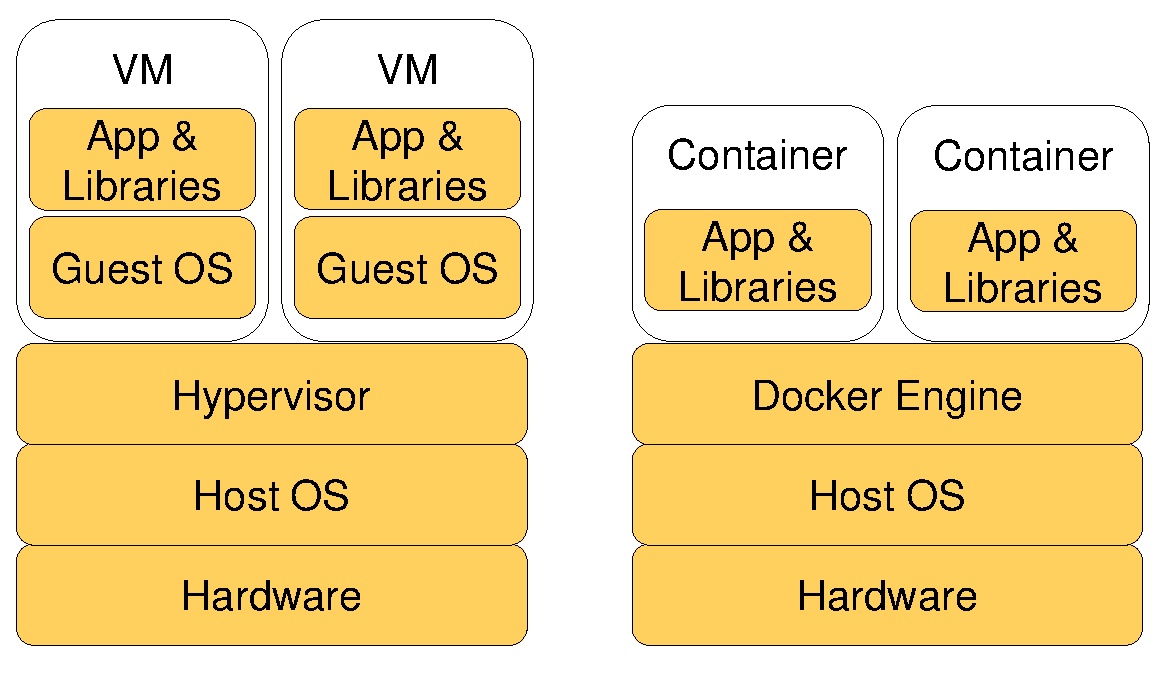
\includegraphics[width=\textwidth]{images/VMxDocker}
		\fonte{Elaborado pelo autor}
	\end{minipage}
\end{figure}

O termo \textit{contêinerização} é a forma popular para se referenciar à virtualização baseada em contêiner, que permite o isolamento de determinados softwares, que são executados dentro do mesmo kernel no sistema operacional Linux. Diferentemente de hipervisores, o Docker não adiciona uma camada virtualização, na qual precisaria carregar um sistema operacional convidado \cite{Zhang2016}. Os contêineres possuem a vantagem de utilizar diretamente os recursos do hospedeiro e não necessitar de tempo de \textit{boot}, além de não possuir o \textit{overhead} de processamento ao traduzir os comandos do sistema operacional convidado para o hospedeiro \cite{Dua2014}.
\begin{comment}
\begin{table}[!ht]
	\caption{Características de VM e contêineres}
	\label{tab:table1}
	\centering
	\resizebox{\textwidth}{!}{%
		\begin{tabular}{|l|l|l|}
			\hline
			\textbf{Parâmetro} &\textbf{Máquinas Virtuais}\ &\textbf{Contêineres}\\
			\hline
			SO Convidado & \begin{tabular}[c]{@{}l@{}}Um hardware virtual é criado para cada\\VM, com um espaço de memória reservado\end{tabular} & \begin{tabular}[c]{@{}l@{}}Todos os convidados compartilham o\\mesmo SO, cada imagem é carregada\\para o espaço de memória do Kernel \end{tabular}\\ \hline
			Comunicação & Feita por dispositivos Ethernet & \begin{tabular}[c]{@{}l@{}} Utilização de mecanismos IPC como sinais,\\sockets, pipes \end{tabular}\\  \hline
			Segurança &\begin{tabular}[c]{@{}l@{}} Depende da implementação do fornecedor\\de hipervisor\end{tabular}& Utilizam mecanismos de controle de acesso\\ \hline
			Desempenho & \begin{tabular}[c]{@{}l@{}}Irá receber uma sobrecarga pelo trabalho\\de tradução de instruções do sistema\\hospedeiro para o convidado\end{tabular}  &\begin{tabular}[c]{@{}l@{}}contêineres fornecem um desempenho\\muito próximo ao nativo em comparação\\ao executado direto no hospedeiro\end{tabular} \\ \hline
			Isolamento &\begin{tabular}[c]{@{}l@{}} Não é possível compartilhar arquivos,\\bibliotecas e execução de programas entre\\as máquinas virtuais  \end{tabular} & \begin{tabular}[c]{@{}l@{}}Subdiretórios podem ser montados e\\compartilhados entre contêineres no mesmo\\hospedeiro \end{tabular} \\ \hline
			Tempo de início & \begin{tabular}[c]{@{}l@{}} Demora o tempo de processo de boot de um \\ sistema operacional \end{tabular} & contêineres não fazem boot de sistema\\ \hline 
			Armazenamento& \begin{tabular}[c]{@{}l@{}}Sistema de arquivos precisa ser\\instalados no convidado além do hospedeiro\end{tabular} & \begin{tabular}[c]{@{}l@{}} O armazenamento em contêineres pode\\ser compartilhado com o hospedeiro \end{tabular} \\ 
			\hline
		\end{tabular}}
		\fonte{\cite{Dua2014}}
\end{table}
\end{comment}
\section{Trabalhos Relacionados}
\label{related}
Nesta seção, será visto um estudo de trabalhos que trazem soluções de elasticidade para aplicações de alto desempenho, bem como estudos comparativos entre a utilização de máquinas virtuais e contêineres, considerados o estado-da-arte na atualidade. Este estudo tem por objetivo confrontar os trabalhos e identificar as lacunas e possíveis melhorias em ambientes elásticos. A seleção de trabalhos relacionados, bem como outras referências, foi realizada através de uma pesquisa em diversas bases de dados de artigos científicos de Ciências Exatas, como o portal da \textit{IEEE Xplore}, \textit{ACM Digital Library} e \textit{Springer Link}, além da bases de dados nacionais, o Portal de Periódicos CAPES/MEC.

Para a realização das pesquisas nessas bases de dados, foram utilizadas buscas com estas principais palavras-chave: \textit{docker virtual machine, container high performance computing, scalability elasticity, hpc application container, virtualization contêineres, cloud computing elasticity}. O resultado dessas pesquisas foi analisado com o intuito de encontrar trabalhos que explorassem a utilização de contêineres em ambientes de computação em nuvem, bem como as alternativas e implementações de elasticidade em aplicações PAD. Sendo assim, verificou-se os 30 primeiros resultados de cada pesquisa e foram descartados resultados focados em áreas muito específicas, ou que não contivessem dados de avaliação de desempenho.

\subsection{Análise do Estado-da-Arte}
\label{state}
O AutoElastic, segundo a definição de \citetexto{7090978}, age como um \textit{middleware} permitindo que aplicações PAD iterativas obtenham vantagem do provisionamento dinâmico de recursos de uma infraestrutura de nuvem sem a necessidade de modificações no código fonte. O AutoElastic possui um protótipo executado pelo autor na plataforma de nuvem OpenNebula e obteve resultados de ganho de desempenho de até 59\% na execução de uma aplicação de integração numérica \textit{CPU-Bound}, quando comparada com outras soluções de elasticidade. 

\citetexto{7562612} fazem um estudo comparativo de máquinas virtuais e contêineres, além de propor um modelo de \textit{deploy} de aplicações distribuídas em contêineres Docker. Para verificar o modelo proposto, foram realizados testes utilizando duas aplicações PAD que requerem grande capacidade computacional, Graph500 e Linpack (HPL). Para manter um base de comparação, foram realizados execuções com processamento nativo, sem adição de camada de virtualização. Os testes executados mediam os custos computacionais dos processos, considerando diversas combinações de instâncias de máquinas virtuais e instâncias de contêineres, sem levar em consideração a elasticidade.

\citetexto{Dua2014} apresentam um estudo sobre como provedores de PaaS (\textit{Platform as a Service})estão utilizando contêineres para encapsular aplicações. O estudo indaga a atual adoção de plataformas baseadas em contêineres e explora diversas implementações de contêineres, entre elas: Linux contêineres, Docker, Warden Container, lmctfy e OpenVZ. A análise foi feita baseada em como cada uma das tecnologias lidam com processos, sistema de arquivos e isolamento de namespaces, dando uma atenção especial à características únicas de cada implementação. Por fim, o trabalho busca fazer uma análise dos fatores que afetam a adoção de contêineres e possíveis funcionalidades que estão em falta para uma nova geração de PaaS.

O estudo de \citetexto{Xavier2013} aborda a utilização de tecnologias de virtualização para aplicações de alto desempenho, alegando que tais tecnologias foram tradicionalmente evitadas ao longo dos anos por sua adição de camadas que comprometem desempenho, o que é crucial para tais aplicações. Porém, como o advento de implementações de virtualização baseada em contêineres, o autor indaga que é possível se obter uma sobrecarga muito pequena com a utilização de tecnologias como Linux VServer, OpenVZ e Linux contêineres (LXC), chegando a um desempenho quase nativo. Para comparação, foi utilizado o Xen, um modelo tradicional de virtualização. Os testes utilizaram programas de avaliação de desempenho de supercomputadores fornecidos pela NASA \cite{NASA2016}. O LXC executou os programas de teste com praticamente o mesmo potencial que a própria máquina, enquanto a implementação utilizando máquina virtual (XEN) obteve uma sobrecarga de aproximadamente 4.3\%.

O trabalho de \citetexto{Zhang2016} aborda a sobrecarga que soluções de hipervisor possuem em relação aos dispositivos de I/O virtualizados. O trabalho apresenta SRV-IOV (\textit{Single Root I/O Virtualization }) para permitir o compartilhamento entre conexões de alto desempenho, como InfiniBand, além de introduzir testes utilizando contêineres, buscando atingir um desempenho mais próximo do nativo. Nos testes, utilizando aplicações de \textit{benchmark} com MPI, as avaliações identificaram que VM com passagem PCI é mais eficiente que VM com SR-IOV habilitado, entretanto, contêineres possuem mais eficiência ao compartilhar recursos de I/O. Em comparação ao desempenho nativo, os testes identificaram uma sobrecarga para contêineres de no máximo 9\% para aplicações PAD.

\citetexto{Adufu2015} conduziram testes para demonstrar que, durante a execução de aplicações científicas em ambientes PAD, o tempo médio de processamento em um sistema com virtualização baseada em contêineres é menor do que o tempo em um sistema baseado em hipervisores, isto devido ao tempo de \textit{start-up}. Para gerar os resultados de comparação, foi utilizado a ferramenta \textit{autodock3}, um programa de simulação de modelagem molecular. Para gerenciar os contêineres, a ferramenta Docker foi utilizada, mostrando um gerenciamento de recursos mais eficiente, até mesmo no cenário em que foi alocado mais memória do que realmente disponível fisicamente para as instâncias em execução. 

\citetexto{Kominos2017} fazem uma análise sobre as opções de provisionamento na plataforma OpenStack, que são: máquinas virtuais, contêineres e \textit{bare-metal} (instalação do zero nas máquinas). As alternativas são comparadas em relação à CPU, networking, operações de I/O e acesso à RAM, além de medição de tempo de \textit{boot}. Contêineres Docker container apresentaram o tempo de início mais rápido, e obteve um desempenho muito próximo do \textit{bare-metal} nos outros quesitos, este que por sua vez, teve os melhores resultados. Em geral, VMs obtiveram os piores resultados, principalmente em relação ao desempenho de múltiplas vCPUs.

O artigo de \citetexto{Molto2017} descreve um \textit{workflow} para permitir a execução de uma aplicação tanto em ambientes virtualizados, como em ambientes baseados em contêineres, o que foi chamado de Infraestrutura Híbrida de Computação Distribuída (IHCD), utilizando ferramentas open-source do projeto INDIGO-DataCloud. O principal problema abordado é a falta de interoperabilidade de uma imagem entre hipervisores (VMs) e contêineres. O resultado é uma ferramenta que permite a criação de um \textit{template} com as especificações necessárias da aplicação e a plataforma OpenNebula cria a imagem e a disponibiliza conforme solicitado (Docker ou VM). O tempo total deste processo para uma aplicação de teste é de 20:48 (minutos:segundos) para VM e 7:25 para Docker.

Para finalizar, \citetexto{Zheng2017} avaliam as diferenças fundamentais entre Docker e máquinas virtuais, contrariando os outros trabalhos relacionados, porquê apresenta situações onde máquinas virtuais podem apresentar um desempenho melhor que contêineres Docker. Nos benchmarks executados, o Docker atingiu um gargalo de velocidade em operações de disco de byte-a-byte, enquanto os testes com VMs atingiram resultados parecidos com o desempenho nativo para resolver o problema N-Queens. Mesmo assim, o trabalho ressalva que as diferenças de \textit{overhead} de desempenho entre os tipos de virtualização ocorrem não somente no modo implementado, como também depende da aplicação em execução. 

\subsection{Discussão e Lacunas}
\label{comparacao}
Na tabela \ref{tab:table2} é feito um resumo dos trabalhos detalhados na subseção \ref{state}, elencando as principais características dos trabalhos conduzidos. Podemos notar que, apesar do trabalho \citetexto{7090978} apresentar um modelo elástico para aplicações PAD, não existem outros estudos que mostrem o comportamento de contêineres sob estas condições. Os demais trabalhos fazem uma análise do desempenho de contêineres, porém sem instanciação dinâmica de contêineres pelo gerenciador, o que daria o aspecto de um sistema elástico.

Os estudos mostrados na tabela \ref{tab:table2} que abordaram a utilização da tecnologia de contêineres, exibem resultados mais favoráveis à estas implementações em comparação ao método tradicionais de virtualização, abordando diversos aspectos inerentes à virtualização de recursos, como operações de I/O, desempenho de memória RAM e consumo de energia. Todos estes são aspectos fundamentais para uma solução de ambiente PAD eficiente. Embora os trabalhos mostrem resultados aplicando programas de \textit{benchmark} para medir o desempenho da infraestrutura, não foi encontrado um estudo que verificasse o desempenho elástico de contêineres para um modelo de provisionamento de recursos de forma dinâmica, como o AutoElastic mostra, utilizando máquinas virtuais.


\begin{table}[!ht]
\centering
\caption{Comparação de trabalhos relacionados}

\label{tab:table2}
\resizebox{\textwidth}{!}{%
\begin{tabular}{lllllll}
\hline
\textbf{Trabalho} & \textbf{Tecnologia}  & \textbf{Elasticidade} & \begin{tabular}[c]{@{}l@{}}\textbf{Base de}\\\textbf{Comparação} \end{tabular}     & \textbf{Métricas}                      & \textbf{Plataforma}  & \textbf{Testes}                                                              \\     \hline
\rowcolor[HTML]{EFEFEF} 
\cite{7090978}       & VM                   & Sim                   & Ubuntu 10.04 &\begin{tabular}[c]{@{}l@{}} desempenho, custo e\\ energia\end{tabular}                                                          & OpenNebula           & cálculo de integrais                                                         \\ 
\cite{7562612}                 & Docker               & Não                   & CentOS 7 3.10         & \begin{tabular}[c]{@{}l@{}} Performance por \\instancias  \end{tabular}                                                        & OpenStack            & \begin{tabular}[c]{@{}l@{}} MPI com Graph500,\\ Linpack\end{tabular}                                                   \\ 
\rowcolor[HTML]{EFEFEF} 
\cite{Xavier2013}                 & \begin{tabular}[c]{@{}l@{}} LXC, OpenVZ,\\ VServer \end{tabular} & Não                   & Ubuntu 10.04               & \begin{tabular}[c]{@{}l@{}}diversos tipos de \\ recursos em único nó\end{tabular} & Não & \begin{tabular}[c]{@{}l@{}}Linpack, STREAM, \\ IOZone, NetPIPE\end{tabular} \\ 
\cite{Zhang2016}                 & Docker               & Não                   & CentOS Linux                    & \begin{tabular}[c]{@{}l@{}}desempenho \\ de comunicação\end{tabular}    & OpenStack            & \begin{tabular}[c]{@{}l@{}}MPI com Graph500,\\ NAS, LAMMPS\end{tabular}     \\ 
\rowcolor[HTML]{EFEFEF} 
\cite{Adufu2015}                 & Docker               & Não                   & Ubuntu 14.04& \begin{tabular}[c]{@{}l@{}}Desempenho de RAM\end{tabular}                & OpenStack            & \textit{autodock3}                                                                    \\ 
\cite{Kominos2017} & Docker& Não & Ubuntu 14.04&\begin{tabular}[c]{@{}l@{}} Desempenho de CPU,\\ rede, RAM e disco\end{tabular}& OpenStack &\begin{tabular}[c]{@{}l@{}} ParallelPXZ,\\ Netperf, SysBench \end{tabular}\\ 
\rowcolor[HTML]{EFEFEF} 
\cite{Molto2017} & Docker & Não & Ubuntu 14.04 & Provisionamento& OpenNebula & Tempo médio \\ 
\cite{Zheng2017} & Docker & Não & Ubuntu 15.10 &\begin{tabular}[c]{@{}l@{}} Desempenho de CPU,\\disco e RAM\end{tabular} & Não &\begin{tabular}[c]{@{}l@{}} Iperf, STREAM,\\HardInfo, Bonnie++\end{tabular}\\ \hline
\end{tabular}}
\fonte{Elaborado pelo autor}
\end{table}

Para o trabalho com aplicações PAD, é muito importante saber todos os aspectos inerentes à infraestrutura que se vai utilizar, como desempenho de CPU, tempo de processamento, energia e custos. Além do hardware, as tecnologias escolhidas devem deixar claro qual seria a mais indicada para o foco da aplicação. Docker contêineres estão sendo cada vez mais adotados, sendo necessário um estudo para entender as diferenças de desempenho sob estes aspectos, contribuindo para decisões de estudos futuros.
%=======================================================================
% Modelo
%=======================================================================
\section{Benchmark DoCB}
\label{model}

Neste capítulo apresentaremos o modelo do Docker Containers Benchmark (DoCB), uma análise de viabilidade de elasticidade em nuvem para contêineres, em comparação ao modelo tradicional, que utiliza máquinas virtuais. Além disto, debateremos em termos gerais as questões de projeto. Na próxima seção \ref{arquitetura}, abordaremos as modificações necessárias no modelo do AutoElastic para suportar este \textit{benchmarking}. A modificação no modelo não é o objetivo principal deste projeto, mas se configura com uma contribuição técnica, permitindo uma maior flexibilidade da ferramenta AutoElastic. 

\subsection{Questões de projeto}
\label{questao}

O DoCB é uma estratégia de \textit{benchmarking}, que segundo \citetexto{6448963}, é uma técnica de executar um programa (ou conjunto), em uma máquina e comparar o desempenho com outra. A técnica em sua origem era voltada para observação topográfica, onde um objeto estacionário era medido para servir de ponto de referência para observações futuras. Em termos relativos, benchmarking serve para identificar ``quais, de várias opções, irão desempenhar melhor em um dado contexto?''. O modelo do DoCB parte de uma observação de um modelo de elasticidade em nuvem utilizando máquinas virtuais, aplicando uma certa carga, para então comparar com a elasticidade com contêineres, dado o cenário de PAD.

Para obter a elasticidade em nuvem, utilizaremos a ferramenta AutoElastic. Nesse caso, iremos estender a ferramenta para permitir a possibilidade de instanciar contêineres além máquinas virtuais, ficando transparente ao usuário essa opção, minimizando a configuração necessária para utilização das opções de virtualização. A elasticidade se dará no momento em que a aplicação decidir adicionar recursos para otimizar a execução das aplicações, utilizando os critérios definidos. Como as imagens de contêineres possuem um tamanho significativamente menor que o de uma máquina virtual, o gerenciador poderá lançar \textit{n} instâncias de contêineres para um mesmo nó, obtendo vantagens ao executar aplicações paralelas. 

O gerenciador AutoElastic foi escolhido por permitir virtualização de acordo com a utilização dos recursos computacionais já alocados. A elasticidade aplicada pelo gerenciador será horizontal, ou seja, a elasticidade é aplicada ao alocar e desalocar recursos virtualizados, e não na configuração de hardware. A métrica utilizada pelo gerenciador será a média de CPU dos contêineres alocados, pois o AutoElastic utiliza a média de CPU das máquinas virtuais para tomada de decisão.

\subsection{Extensão da Arquitetura do AutoElastic}
\label{arquitetura}
Este trabalho parte da implementação do modelo AutoElastic para propor uma modificação em sua arquitetura, acrescentando a possibilidade de utilizar contêineres ao invés de máquinas virtuais. O AutoElastic é um \textit{middleware}, que permite que o usuário possa obter elasticidade para suas aplicações, sem depender de alterações no código-fonte. Operando no nível de PaaS, o modelo permite que aplicações iterativas obtenham elasticidade através de operações de alocação e consolidação de instâncias de máquinas virtuais em nós físicos. O \textit{framework} atual é composto por um Gerenciador, um componente independente da infraestrutura, não interferindo no resultado da execução e podendo gerenciar os recursos remotamente, através do acesso de um computador \textit{frontend} da Nuvem de computadores.

A figura \ref{fig:arquitetura} mostra como é a arquitetura do modelo adaptado. Cada nó possui um gerenciador de Docker contêineres, além da implementação corrente de hipervisor. Aqui, utilizaremos o termo Unidade de Processamento Virtualizada (UPV), que pode se referir tanto para uma máquina virtual, quanto um contêiner. O número de UPVs pode partir de 1 por nó, a partir do UPV do processo mestre da aplicação, até vários UPVs por nó, definido pelo usuário do gerenciador \cite{6307065}. O gerenciador analisa periodicamente as instâncias de UPVs que estão ativas, e verifica se é necessário um adição ou remoção de recursos, dependendo da configuração de \textit{threshold}. No modelo proposto, o usuário pode definir o número minimo e máximo de UPVs por nó e quantos poderão operar na execução da aplicação. Ainda, a arquitetura garante que a aplicação em execução não tenha o seu desempenho afetado pela adição ou remoção de recursos, pois o gerenciador atua de forma isolada da Nuvem de computadores. 
\begin{figure}[ht!]
	\caption{Infraestrutura do Modelo. Aqui, \textit{n} representa o número de nós disponíveis, e \textit{m} o número de Unidades de Processamento Virtualizadas (UPV - seja uma máquina virtual ou contêiner).}
	\label{fig:arquitetura}
	\centering%
	\vspace{-0.5\baselineskip}
	\begin{minipage}{0.8\textwidth}
		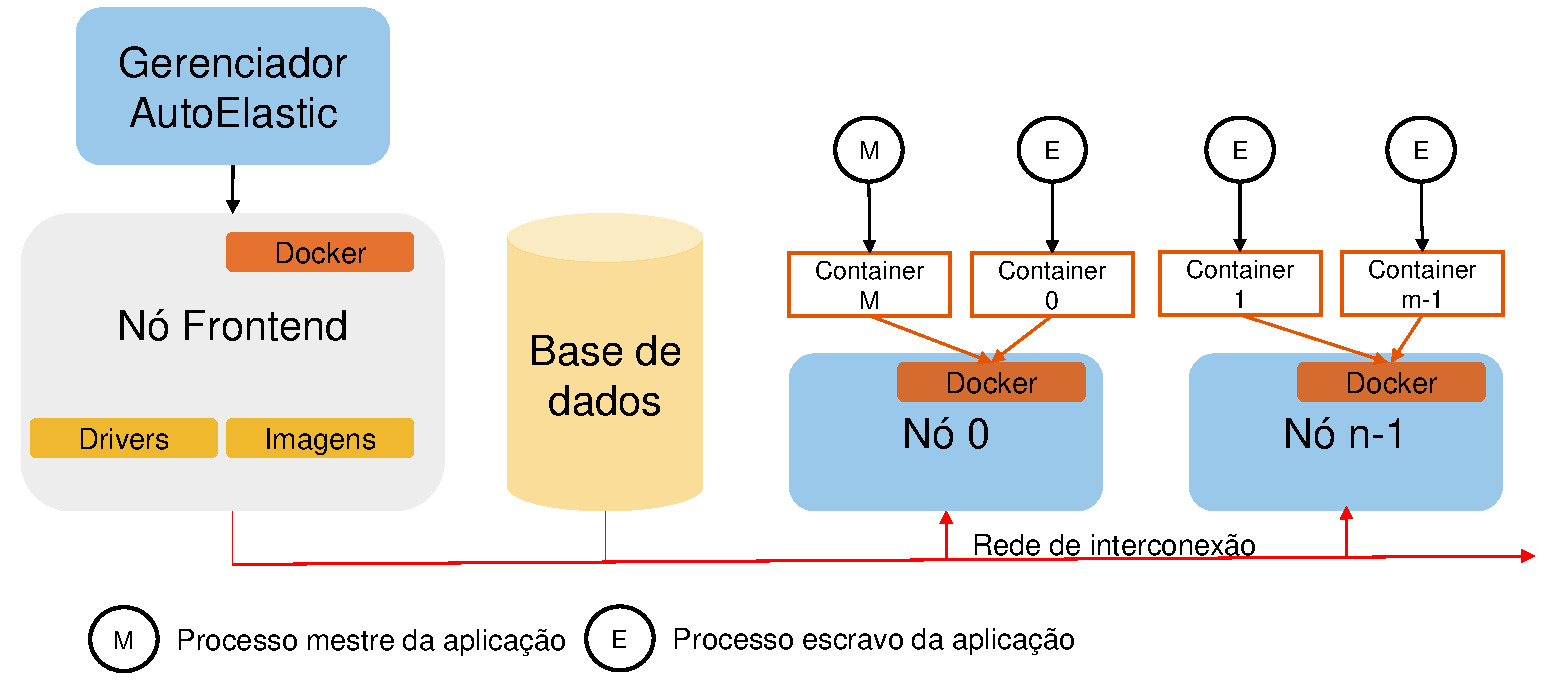
\includegraphics[width=\textwidth]{images/arquitetura}
		\fonte{Elaborado pelo autor}
	\end{minipage}
\end{figure}
A base de dados mostrada na figura \ref{fig:arquitetura} é utilizada para armazenar as imagens utilizadas pelo nó \textit{frontend}, além de permitir um espaço de comunicação entre o gerenciador e as instâncias de UPVs em execução, sendo este espaço acessível apenas pelos computadores da Nuvem. A utilização de uma área compartilhada, para comunicação entre computadores virtualizados é uma prática comum, quando se falando de nuvens privadas. No contexto de Docker, a base de dados é um banco local \textit{Docker Repository} e a área de dados comum é montada pelos contêineres utilizando a ferramenta de \textit{volumes}, que monta um diretório compartilhado.

\subsection{Elasticidade}
As aplicações de PAD normalmente lidam com computação intensiva, por esse motivo, iremos nos concentrar apenas na métrica de CPU para tomada de decisão. O Gerenciador captura periodicamente os valores de carga de CPU dos objetos virtualizados (máquina virtual ou contêiner) que estão executando os processos. É feita uma média desses valores e estes são armazenados juntamente com coletas operações anteriores para realizar o cálculo de carga geral. O valor resultante do cálculo é avaliado conforme regras definidas de \textit{threshold} superior e inferior, que são definidos por valores de 0\% a 100\% respectivamente. O AutoElastic possui em sua implementação algumas opções de algoritmo de avaliação, entre elas o algoritmo que opera segundo o conceito \textit{Aging}. Segundo \citetexto{Tanenbaum03}, a técnica utiliza uma suavização exponencial simples, aplicando maior peso para a última coleta para definir a carga.

\begin{comment}
O AutoElastic possui em sua implementação algumas opções de algoritmo de avaliação, entre elas o algoritmo que opera segundo o conceito \textit{Aging}. Segundo \citetexto{Tanenbaum03}, a técnica utiliza uma suavização exponencial simples, aplicando maior peso para a última coleta para definir a carga. O algoritmo permite suavizar picos de carga (superior e inferior), evitando operações de elasticidade desnecessárias, causadas por falso-positivos em termos de atingir um \textit{threshold}. Podemos ver, na Figura~\ref{fig:aging}, um caso simples onde as operações de elasticidade ocorreriam se fosse considerado apenas a carga real medida, porém, com a técnica de \textit{Aging}, evitamos estas operações de elasticidade. Assim, foi escolhido esse algoritmo para evitar ruídos nas leituras que possam prejudicar a execução eficiente da aplicação. Os \textit{thresolds} superior e inferior são fixos, sendo esses informados previamente antes do iniciar o monitoramento.

\begin{figure}
	\caption{Utilização da técnica de \textit{Aging} para alocar e desalocar recursos de de forma suavizada}
	\label{fig:aging}
	\centering%
	\vspace{-0.75\baselineskip}
	\begin{minipage}{0.75\textwidth}
		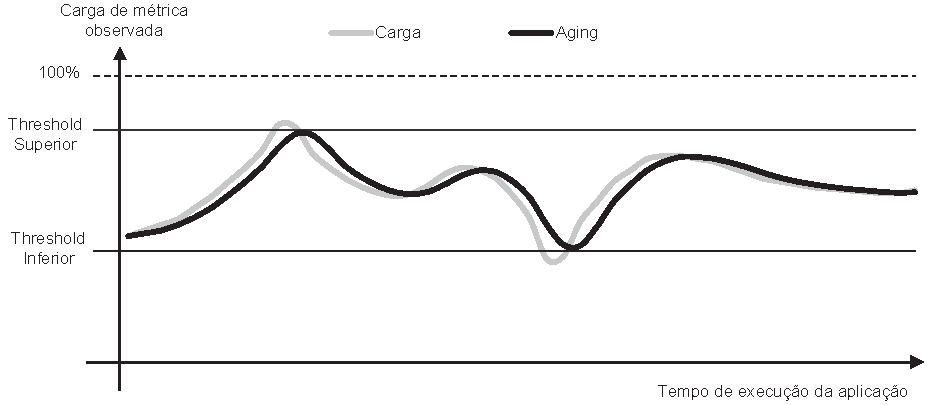
\includegraphics[width=\textwidth]{images/aging}
		\fonte{\cite{7090978}}
	\end{minipage}
\end{figure}
\end{comment}
\subsection{Modelo do benchmarking}

Para poder avaliar o desempenho dos contêineres com operações de elasticidade, será criada uma base de comparação, que se configura por uma execução do processo utilizando máquinas virtuais, e o AutoElastic como Gerenciador. Nessa execução, utilizaremos o hipervisor KVM\footnote{https://www.linux-kvm.org} para virtualização. A Figura \ref{fig:flow} demonstra o processo de avaliação do \textit{benchkmark} para uma aplicação.

O processo se inicia na configuração do Gerenciador para lidar com máquinas virtuais. A configuração envolve a imagem que irá rodar a aplicação, com especificação de CPU e memória alocados, bem como a rede que irá utilizar. Inicia-se então, a aplicação e o monitoramento da nuvem, que identifica os recursos ativos e os processos em execução. A coleta de dados é feita no próximo passo, que a cada intervalo de 15 segundos, avalia a carga de CPU das instâncias alocadas, utilizando estes dados para a decisão. Os \textit{threshold} superior e inferior são verificados para decidir alocar ou desalocar recursos para a aplicação. No caso de alocar, um número \textit{x} de instâncias (VM ou contêiner) são instanciados para uma nova máquina carregada e a carga da aplicação é distribuída entre todos os recursos disponíveis.

\begin{figure}[ht!]
	\caption{Processo de coleta de dados do benchmarking, avaliando a execução de uma aplicação com máquinas virtuais e contêineres}
	\label{fig:flow}
	\centering%
	\vspace{-0.75\baselineskip}
	\begin{minipage}{0.9\textwidth}
		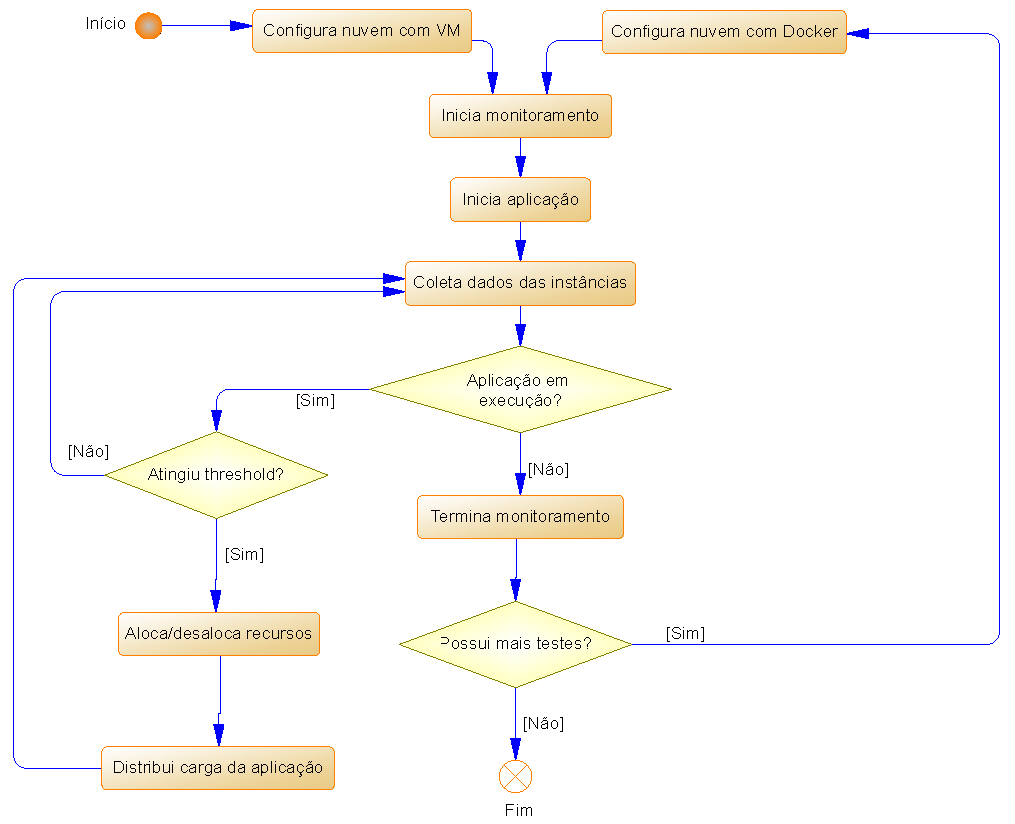
\includegraphics[width=\textwidth]{images/flow_modelo}
		\fonte{Elaborado pelo autor}
	\end{minipage}
\end{figure}

Na coleta de dados também é verificado se a aplicação já terminou o processamento, finalizando esta etapa do processo e iniciando a etapa de execuções com contêineres, que pode vir a ser de \textit{n} iterações, dependendo das configurações de \textit{templates} disponíveis. A ferramenta ONEDock\footnote{https://github.com/indigo-dc/onedock} é utilizada para configurar a nuvem para suportar contêineres Docker. O processo acaba quando se esgota as iterações da bateria de testes.

Uma imagem de contêiner Docker é criada a partir de um arquivo chamado \textit{Dockerfile}, que contém instruções de configuração ao criar a imagem. Esta imagem pode ser extremamente pequena, se comparada à uma imagem virtualizada tradicional, ocupando poucos megabytes. Outra peculiaridade de contêineres é que estes não possuem configuração de limitação de recursos por padrão, ou seja, um contêiner irá utilizar tanta CPU e memória da máquina, quanto for disponibilizado pelo agendador do \textit{kernel}. Esta característica nos permite criar um \textit{template} diferente para os contêineres, sem limitação de recursos, diferentemente de máquinas virtuais, que precisam ter definido o quanto de memória e CPU da máquina que irão utilizar. 

Para cada execução da aplicação com contêineres, iremos configurar sempre um par de \textit{templates}:
\begin{itemize}
	\item Rígido: Ao iniciar um contêiner, iremos especificar quantos ciclos de máquina da CPU (subconjunto de MHz da capacidade teórica do processador em questão) o contêiner poderá utilizar, mesmo comportamento que a máquina virtual.
	\item Flexível: Iremos iniciar o contêiner em um processador, sem especificar limite de recursos. Os ciclos de máquina da CPU serão obtidos sob demanda, sendo concorrente com outros contêineres e processos, sem isolamento.
\end{itemize} 

Sendo assim, podemos explorar vários cenários com contêineres, após termos o cenário base com máquinas virtuais. O modelo do benchmarking especifica a abordagem mostrada na Figura \ref{fig:modelo}. Nela podemos identificar que diferentes números de instâncias de contêineres podem ser exploradas para popular os nós nos cenários, sendo que sempre será executado uma vez com formato Rígido e outro Flexível.

\begin{figure}[ht!]
	\caption{Modelo de cenários para execução do benchmarking, onde n representa o limite de cenários para contêineres}
	\label{fig:modelo}
	\centering%
	\vspace{-0.75\baselineskip}
	\begin{minipage}{0.7\textwidth}
		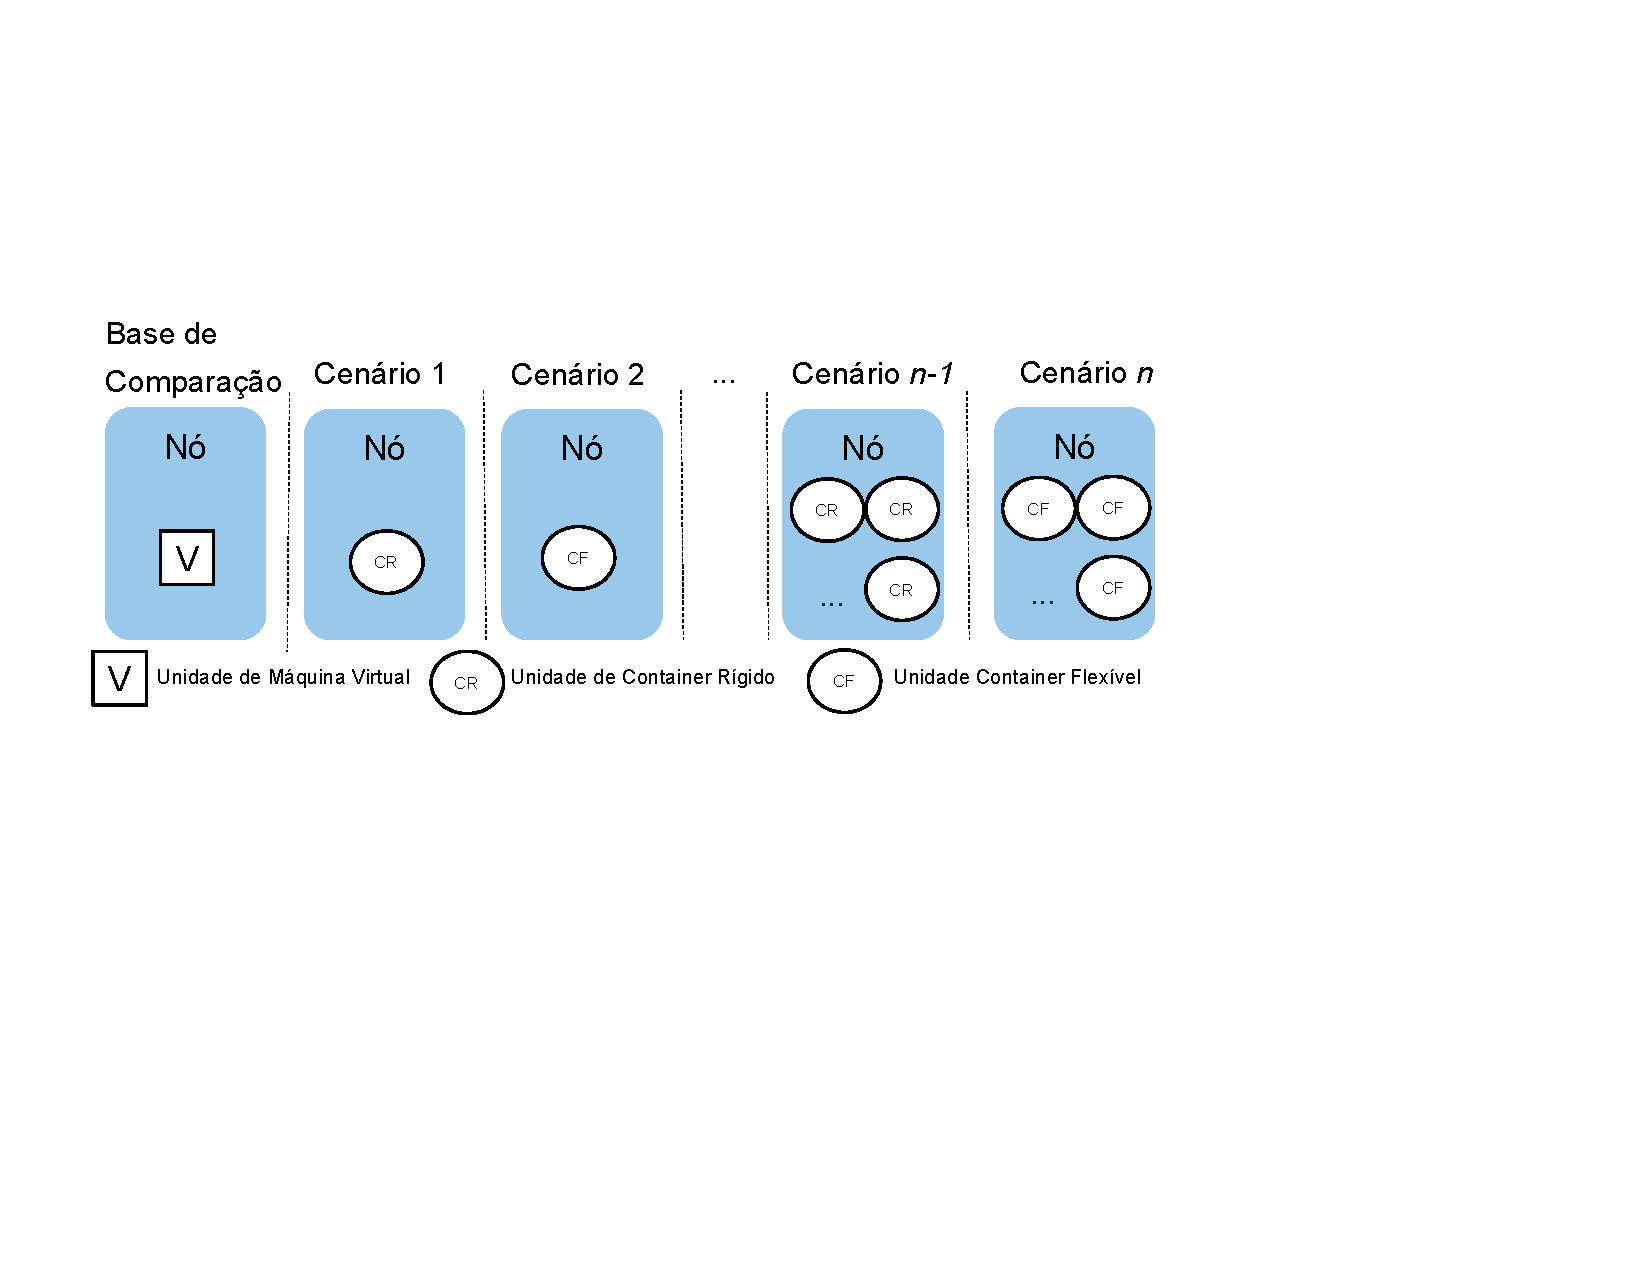
\includegraphics[width=\textwidth]{images/cropped_cenarios}
		\fonte{Elaborado pelo autor}
	\end{minipage}
\end{figure}

\section{Metodologia de Avaliação}
Nesta seção, será apresentado as modificações necessárias no AutoElastic para suportar contêineres. Após isto, será mostrado como o modelo do \textit{benchmarking} foi implementado. As especificações da implementações englobam a aplicação utilizada, os cenários que foram escolhidos e detalhes técnicos da infraestrutura utilizada.

\subsection{Implementação}
\label{prototype}

Para a execução dos experimentos em nuvem, utilizaremos o protótipo desenvolvido por Facco \citetexto{7090978}, que consiste de uma aplicação em Java para gerenciamento de elasticidade, o AutoElastic. O modelo será estendido, passando a considerar a utilização de contêineres. O protótipo atual consiste de uma ferramenta que gerencia uma nuvem OpenNebula, sendo o controle do ambiente realizado através de uma API em Java que o \textit{middleware} OpenNebula oferece, como por exemplo, a criação de máquinas virtuais dentro da Nuvem. 

O ONEDock é um conjunto de extensões para o OpenNebula para utilização de Docker contêineres como entidades de primeira classe, assim como se fossem máquinas virtuais leves. Para tal, Docker é configurado para atuar como um hipervisor, comportando-se então, como o KVM faz no contexto de OpenNebula \cite{onedock2015}. Este conjunto de ferramentas é open-source, o que possibilitou a codificação de características não suportadas pela distribuição atual da ferramenta, como por exemplo a especificação de CPU e memória limitada para o contêiner.

\subsection{Cenários de avaliação}
\label{cenarios}

Para a execução dos cenários de teste, utilizaremos a aplicação desenvolvida por \citetexto{7090978}, o programa consiste de um algoritmo para rodar cálculos de integrais em uma rede privada, seguindo o modelo mestre-escravo, sob diferentes tipos de comportamento de carga de computação, no nosso caso, utilizaremos a carga ascendente e descendente. A aplicação realiza cálculos numéricos e distribui porções de trabalho para cada nó, interligados por MPI (\textit{Message Passing Interface}). O processo mestre fica ciente de novos nós disponíveis utilizando um sistema de comunicação de troca de arquivos de texto, disponibilizados pela aplicação AutoElastic durante as operações de elasticidade. O objetivo da aplicação é puramente demonstrar as operações de elasticidade do Gerenciador, considerando as variações de carga e o impacto do assincronismo no desempenho de aplicações.

\subsubsection{Definição dos testes}

O processo inicia com uma execução da aplicação utilizando máquinas virtuais. Para tal, dois templates de imagens foram configurados com o sistema operacional Ubuntu 10.10, sendo o mestre provido com 1 unidade de CPU e 1GB de RAM, além do template escravo com 1 unidade de CPU e 2GB de RAM, desta forma, cada vez que for solicitado por um recurso adicional de computação, uma unidade escravo é carregada para um dos nós de computação, ocupando 1 dos cores de CPU e metade da memória RAM disponível.

A execução da aplicação paralela com configuração de 2 VMs por nó (1 VM por core) é considerada otimizada, já que cada core se responsabiliza por um processo \cite{7090978}. Porém, não sabemos se a mesma regra se aplica ao cenário de contêineres, por serem processos mais leves que uma máquina virtual, é possível que um número maior de contêineres por nó tenha um desempenho melhor. Tendo em vista isto, criamos os cenários de acordo com a tabela \ref{tab:table3}.

No cenário 1 da tabela, temos o que seria uma configuração considerada equivalente ao definido para o cenário de máquinas virtuais, ou seja, 2 contêineres por operação, sendo cada um com 1 core da CPU e 2GB de memória RAM. O cenário 2 também inicia o processo com 2 contêineres na máquina, porém sem especificação de recursos, deixando a máquina alocar processamento para os processos, conforme necessário. Foram criados outros 2 cenários para avaliar a capacidade de paralelização dos contêineres, ambos com suas variações de Rígido e Flexível em relação à limitação de recursos.

\begin{table}[ht!]
\centering
\caption{Cenários de contêineres}
\label{tab:table3}
\begin{tabular}{lllll}
\hline
\textbf{Cenário} & \textbf{Escravos Iniciais} & \textbf{CPU alocada} & \textbf{RAM alocada (MB)} & \begin{tabular}[c]{@{}l@{}}\textbf{contêineres}\\\textbf{por operação}\end{tabular}\\ \hline
\rowcolor[HTML]{EFEFEF} 
1& 2 & 1 & 2048  & 2  \\ 
2& 2& Não & Não& 2\\ 
\rowcolor[HTML]{EFEFEF} 
3 & 4& 0.5   & 1024& 4\\ 
4 & 4& Não  & Não & 4\\ 
\rowcolor[HTML]{EFEFEF} 
5& 8 & 0.25 & 512  & 8  \\ 
6& 8& Não & Não& 8\\ \hline
\end{tabular}
\end{table}

Na Figura \ref{fig:deploy} podemos identificar como o gerenciador trata cada uma das variações de cenários de \textit{deploy}. O \textit{deploy} 1 é a primeira etapa do processo, entregando duas máquinas virtuais para o recurso alocado. Posteriormente, temos o \textit{deploy} 2, no qual a mesma quantidade de contêineres é entregue para uma nova máquina alocada, este processo ocorre tanto para o modo Rígido quanto para o modo Flexível de limitação de processamento (lembrando que o Rígido é o equivalente à máquinas virtuais). Na sequência, o \textit{deploy} 3 é executado, entregando 4 contêineres para uma máquina alocada, novamente com os dois modos (Rígido e Flexível). Finalmente, um último teste é executado entregando 8 contêineres por operação de elasticidade.

\begin{figure}[ht!]
	\caption{Cenários de \textit{deploy} de instâncias de máquinas virtuais e contêineres para uma mesma máquina}
	\label{fig:deploy}
	\centering%
	\begin{minipage}{0.8\textwidth}
		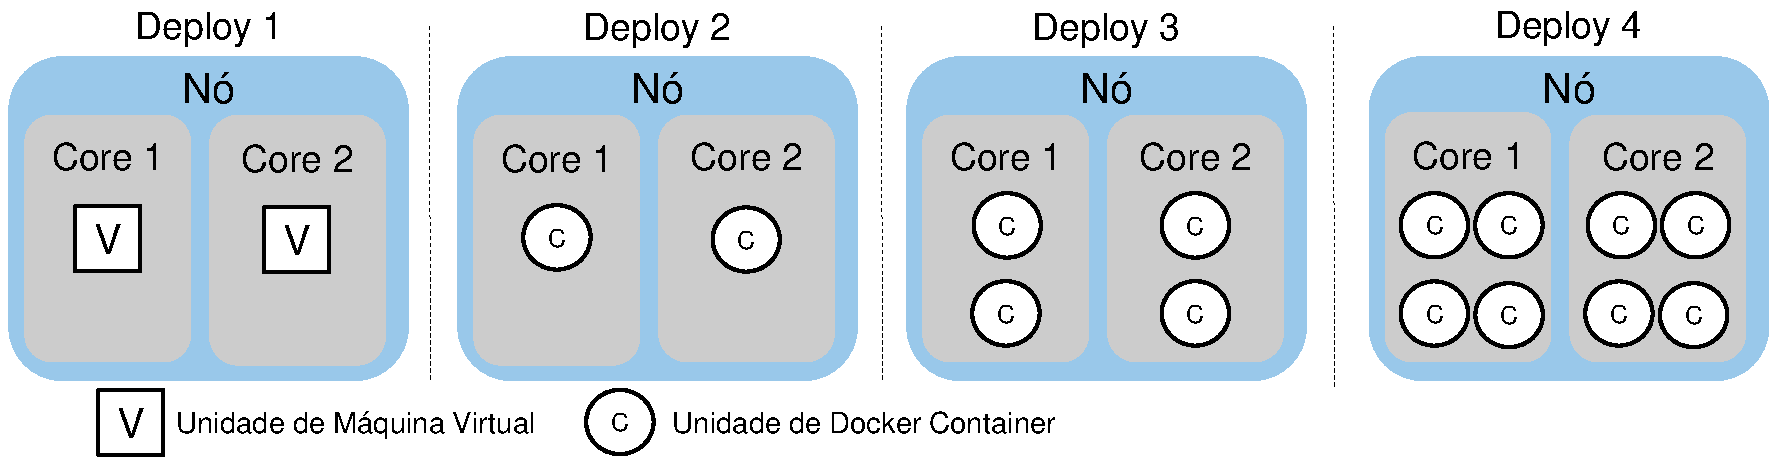
\includegraphics[width=\textwidth]{images/deploy}
		\fonte{\cite{whitepaperDocker2016}}
	\end{minipage}
\end{figure}

\subsubsection{Infraestrutura}

Como infraestrutura de nuvem, utilizaremos o ambiente disponibilizado pela Universidade do Vale do Rio dos Sinos, localizado no laboratório C01 413 do Programa de Pós-Graduação em Computação Aplicada (PIPCA). O laboratório conta com 18 computadores, interconectados através de uma rede 100Mbps, sendo a configuração de cada um deles uma memória de 4 GB, além de processadores de dois núcleos de 2.9 GHz. Porém, para fins de teste de cenários específicos deste trabalho, 5 máquinas do laboratório foram configuradas para serem utilizadas. A plataforma de nuvem OpenNebula será instalada nesta rede de computadores para a execução do protótipo, sendo que uma das máquinas será utilizada como nó \textit{Front-End}. 
A versão 1.1 do ONEDock tem suporte mínimo para a distribuição 4.14 do OpenNebula, portanto esta também teve que ser instalado. Além disto,a versão 1.9 do Docker foi escolhida por ser a versão para qual o ONEDock 1.1 possui suporte até o presente momento. 

\subsection{Métricas e Parâmetros}

De forma a contemplar os trabalhos relacionados, os valores 80\% e 40\% foram escolhidos para os thresholds superior e inferior. Como métricas de desempenho, foram escolhidos o tempo total de execução, a energia gasta e o custo de processamento. A energia é avaliada de acordo com o número de máquinas em cada observação, podemos ver na equação \ref{eq:1} , onde \(i\) é número de máquinas físicas no tempo \(T(i)\).  O custo é mostrado na Equação \ref{eq:2}, que é uma função de adaptação do custo de computação paralela para ambientes elásticos \cite{Barry2004}. O objetivo desta métrica é identificar se uma determinada configuração é viável em termos de custo mas se pode não ser aceitável em questão de tempo total de execução. 

\begin{equation}
\label{eq:1}
Energia = \sum_{i=1}^{n}{(i \times T(i))}
\end{equation}
\begin{equation}
\label{eq:2}
Custo = Tempo \times Energia
\end{equation}

\section{Resultados}
\label{avaliacao}
Nesta seção serão apresentados os resultados dos testes executados conforme descrito anteriormente. Inicialmente é possível observar que a Figura~\ref{fig:trend_asc} mostra os resultados obtidos durante o teste com carga ascendente. Como pode ser observado (a), quando a operação de elasticidade é disparada para a infraestrutura com máquinas virtuais - no threshold de 80\% - ocorre um tempo de espera de 180 segundos até que as 2 novas máquinas virtuais estejam prontas para uso da aplicação. Este mesmo comportamento ocorre para as outras duas operações subsequentes de elasticidade no mesmo teste.

Ao utilizar 2 contêineres por operação de elasticidade, com o modelo Rígido de CPU (b), é possível observar que a operação de elasticidade (instanciar 2 novos contêineres) demorou 30 segundos, um número muito menor em comparação com as máquinas virtuais. Além disto, é importante observar que: 2 operações de elasticidade não ocorreram - a aplicação rodou em apenas 2 nós, ao invés de 4 - e que mesmo assim, o tempo total de execução foi de 380 segundos a menos. No teste com 2 contêineres utilizando o modelo Flexível de CPU (c), não foi observado diferença nas operações de elasticidade, mas como esperado, ocorreu um tempo menor de execução da aplicação, em torno de 45 segundos. Quando se aumentou o número de contêineres por operação (d)(e)(f)(g), notou-se um aumento linear, tanto na duração da operação de elasticidade, como no tempo total da aplicação. 

Em todas as operações com contêineres, percebeu-se uma diferença significativa em relação ao teste com VM's. O que corrobora com a questão do \textit{overhead} na utilização de máquinas virtuais, conforme os argumentos dos trabalhos relacionados. Porém, como no nosso caso, esse \textit{overhead} pode ser a diferença entre ser necessário alocar um recurso a mais ou não. É possível observar essa sobrecarga logo no começo das execuções: para o teste com máquinas virtuais (a), a carga chega aos 40\% logo nos 45 segundos de execução, já para todas as outras execuções com contêineres, isto não ocorre antes dos 130 segundos de execução.

\begin{figure}[ht!]
\centering
\caption{Tendência de tempo de execução de aplicação \textbf{ascendente}, variando o número de instâncias virtualizadas por nó alocado}
\label{fig:trend_asc}
\vspace{-0.4\baselineskip}
\subfloat[2 VM's por nó]{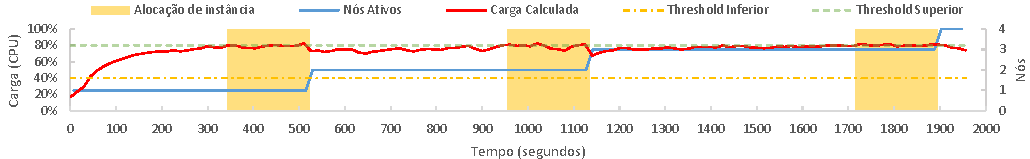
\includegraphics[width= 14cm]{charts/asc2VMFixo.pdf}}\\
\label{fig:trend_asc_a}
\vspace{-0.4\baselineskip}
\subfloat[2 contêineres por nó (CPU Rígido)]{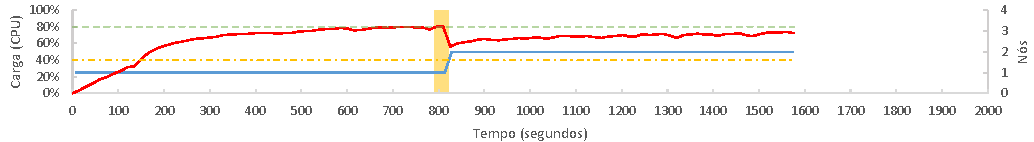
\includegraphics[width= 14cm]{charts/asc2contFixo.pdf}}\\
\vspace{-0.4\baselineskip}
\subfloat[2 contêineres por nó (CPU Flexível)]{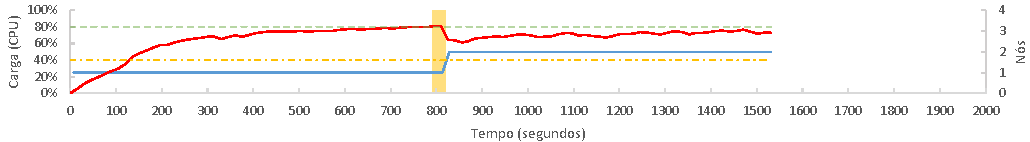
\includegraphics[width= 14cm]{charts/asc2contFlex.pdf}}\\
\vspace{-0.4\baselineskip}
\subfloat[4 contêineres por nó (CPU Rígido)]{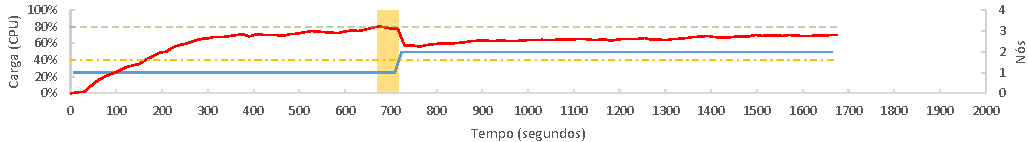
\includegraphics[width= 14cm]{charts/asc4contFixo2.pdf}}\\
\vspace{-0.4\baselineskip}
\subfloat[4 contêineres por nó (CPU Flexível)]{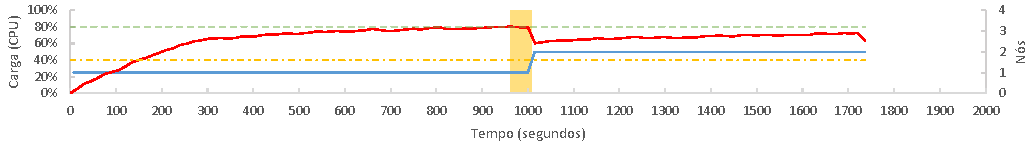
\includegraphics[width= 14cm]{charts/asc4contFlex.pdf}}\\
\vspace{-0.4\baselineskip}
\subfloat[8 contêineres por nó (CPU Rígido)]{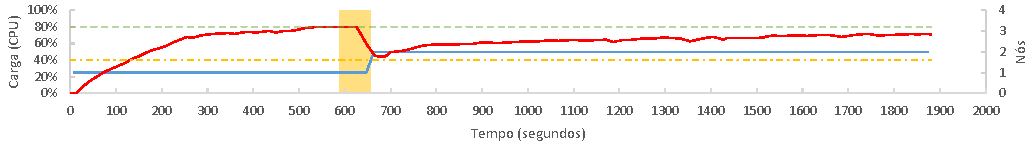
\includegraphics[width= 14cm]{charts/asc8contFixo.pdf}}\\
\vspace{-0.4\baselineskip}
\subfloat[8 contêineres por nó (CPU Flexível)]{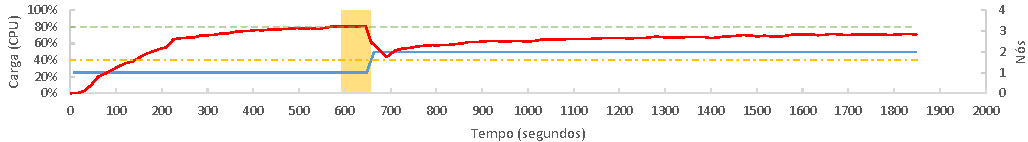
\includegraphics[width= 14cm]{charts/asc8contFlex.pdf}}\\
\fonte{Elaborado pelo autor.}
\end{figure}

Na Figura \ref{fig:trend_des} é possível observar as técnicas de virtualização trabalhando com carga descendente. Neste cenário, o mesmo comportamento de carga se repete, exigindo mais processamento com máquinas virtuais. No teste com operações de 2 VM's (a), temos 3 operações de elasticidade, praticamente em sequência, ficando com 4 nós alocados. Posteriormente, a carga fica abaixo do threshold inferior (40\%) e a desalocação de 2 máquinas virtuais é acionada. O tempo de desalocar os recursos tende a ser o mesmo utilizando contêineres (b), demorando em média de 15 a 30 segundos, o que se refere ao tempo médio de 1 a 2 verificações do gerenciador. 

\begin{figure}[ht!]
\centering
\caption{Tendência de tempo de execução de aplicação \textbf{descendente}, variando o número de instâncias virtualizadas por nó alocado, e atingindo \textit{thresholds} superior e inferior}
\vspace{-0.4\baselineskip}
\subfloat[2 VM's por nó]{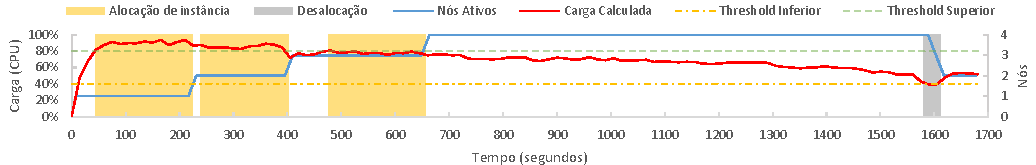
\includegraphics[width= 14cm]{charts/desVMFixo.pdf}}\\
\vspace{-0.4\baselineskip}
\subfloat[2 contêineres por nó (CPU Rígido)]{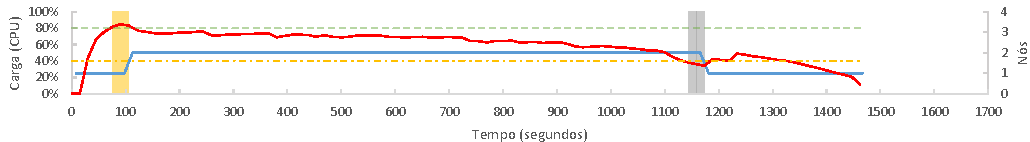
\includegraphics[width= 14cm]{charts/des2contFixo.pdf}}\\
\vspace{-0.4\baselineskip}
\subfloat[2 contêineres por nó (CPU Flexível)]{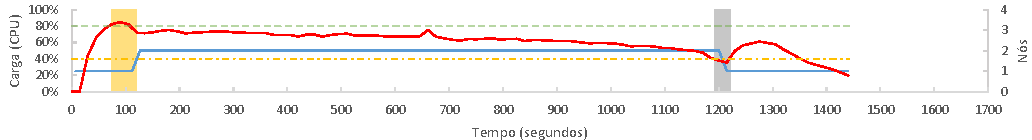
\includegraphics[width= 14cm]{charts/des2contFlex.pdf}}\\
\vspace{-0.4\baselineskip}
\subfloat[4 contêineres por nó (CPU Rígido)]{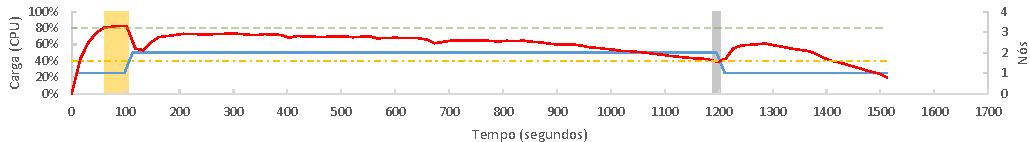
\includegraphics[width= 14cm]{charts/des4contFixo.pdf}}\\
\vspace{-0.4\baselineskip}
\subfloat[4 contêineres por nó (CPU Flexível)]{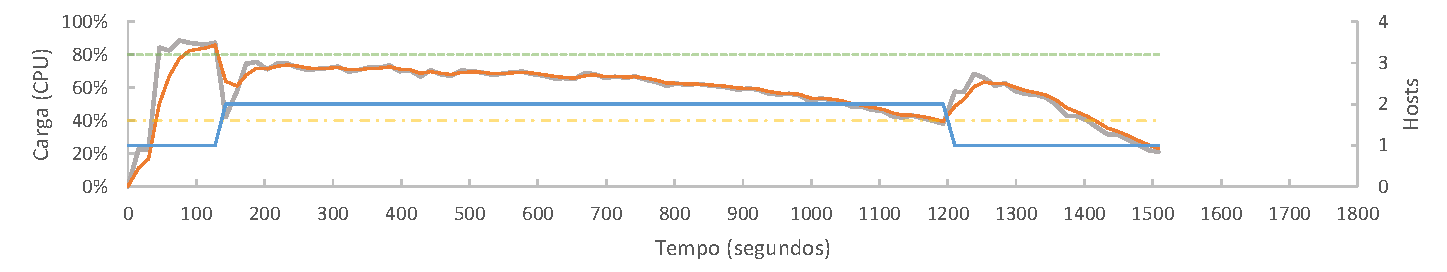
\includegraphics[width= 14cm]{charts/des4contFlex.pdf}}\\
\vspace{-0.4\baselineskip}
\subfloat[8 contêineres por nó (CPU Rígido)]{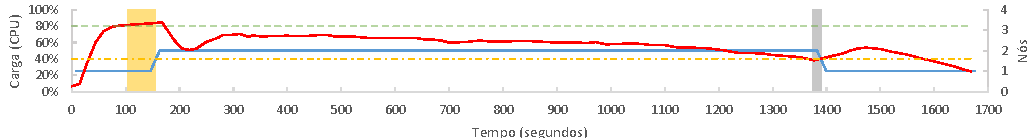
\includegraphics[width= 14cm]{charts/des8contFixo.pdf}}\\
\vspace{-0.4\baselineskip}
\subfloat[8 contêineres por nó (CPU Flexível)]{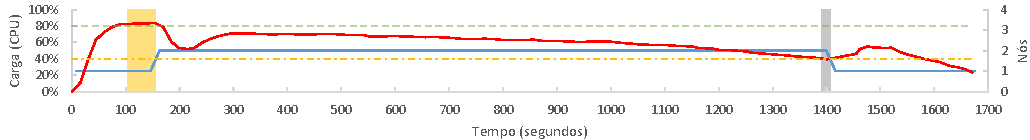
\includegraphics[width= 14cm]{charts/des8contFlex.pdf}}\\

\label{fig:trend_des}
\end{figure}


É possível notar que, assim como no teste com carga ascendente, a execução com 2 contêineres com CPU Flexível (c), é a que apresentou um menor tempo total de execução, mesmo com apenas 1 adição de nó, gerando uma diferença de aproximadamente 300 segundos. Esta execução, assim como as outras com contêineres, finalizou com carga de CPU abaixo dos 40\%, porém a operação de desalocação não ocorre, pois foi configurado para possuir no mínimo um nó executando a aplicação até ela terminar o processamento.




\subsection{Análise}
A Figura~\ref{fig:perf_asc} mostra um comparativo das métricas coletadas de cada estratégia de virtualização durante os testes executados. Conforme já destacado nos resultados anteriores, as métricas confirmam o desempenho superior para a virtualização com contêineres para as aplicações de carga ascendente e descendente. Como pode ser observado na Figura~\ref{fig:perf_asc}, tanto o tempo total de execução, quando a energia calculada, são menores para os contêineres, o que reflete num valor de custo calculado bastante discrepante. 

No cálculo de custo para a aplicação ascendente (c), a execução com 2 contêineres com CPU Flexível apresentou uma diferença de 59\% em relação ao teste com 2 máquinas virtuais. Se formos comparar os dois modelos de CPU (Rígido e Flexível) para uma mesma execução de contêineres, poderemos notar um valor de 6,5\% menor para o teste de 2 contêineres com CPU Flexível em comparação ao teste com 2 contêineres com CPU Rígido. No cálculo de custo para a aplicação descendente (f), o teste com 2 contêineres e CPU Flexível mostrou um ganho de 60\% em comparação à execução com 2 máquinas virtuais. A grande diferença de custo , no casos destes testes, se dá principalmente pelo maior consumo de energia pelas máquinas virtuais, o fato de ter sido necessário dois nós a mais para cada tipo de aplicação, influenciou num custo calculado muito maior para esta estratégia de virtualização. 

\begin{figure}[ht!]
\centering
\caption{Desempenho para aplicação ascendente (cont. R. abrevia para contêineres rígidos e cont. F. para contêineres flexíveis para limite de CPU utilizada)}%
\label{fig:perf_asc}%
\subfloat{
\includegraphics{charts/cropped_legendas.pdf}}\\
\vspace{-0.7\baselineskip}
\setcounter{subfigure}{0}%
\subfloat[][]{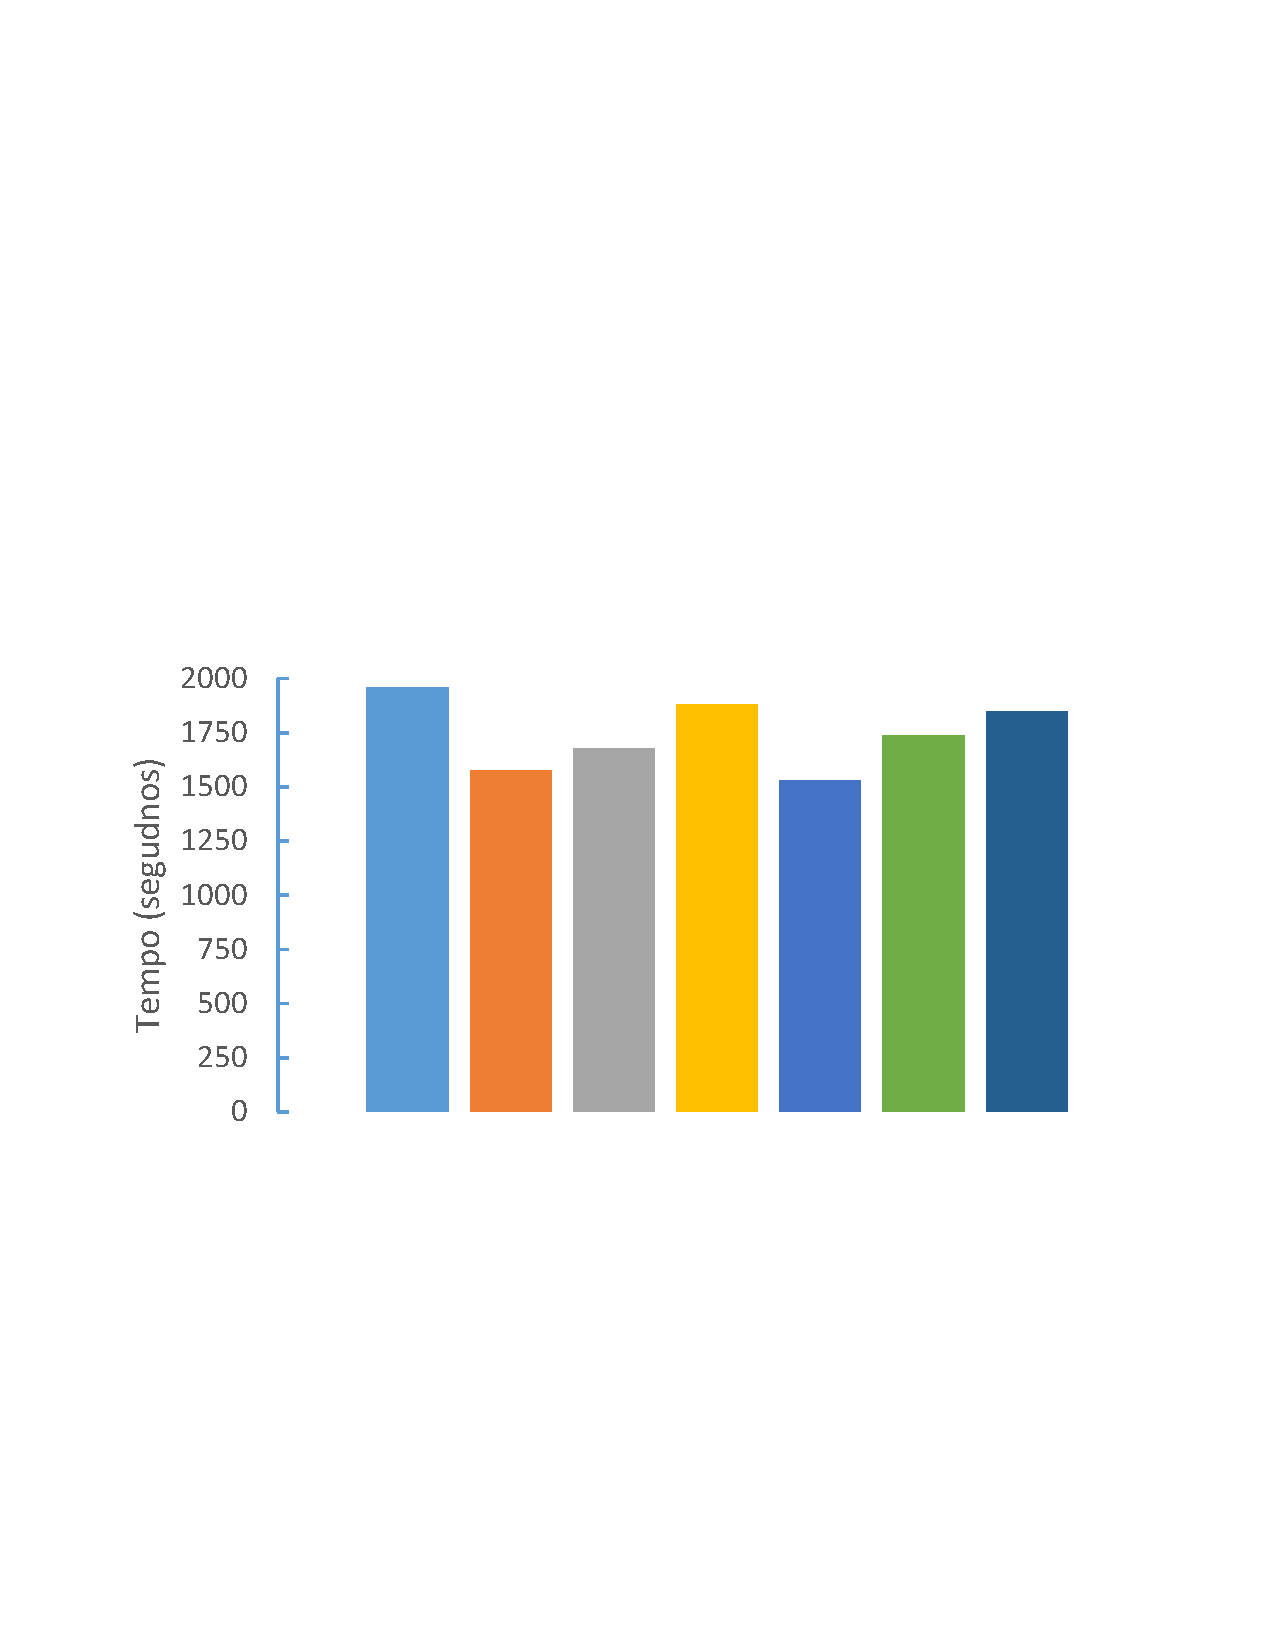
\includegraphics[width= 5cm]{charts/tempo_asc.pdf}}\
%\qquad
\subfloat[][]{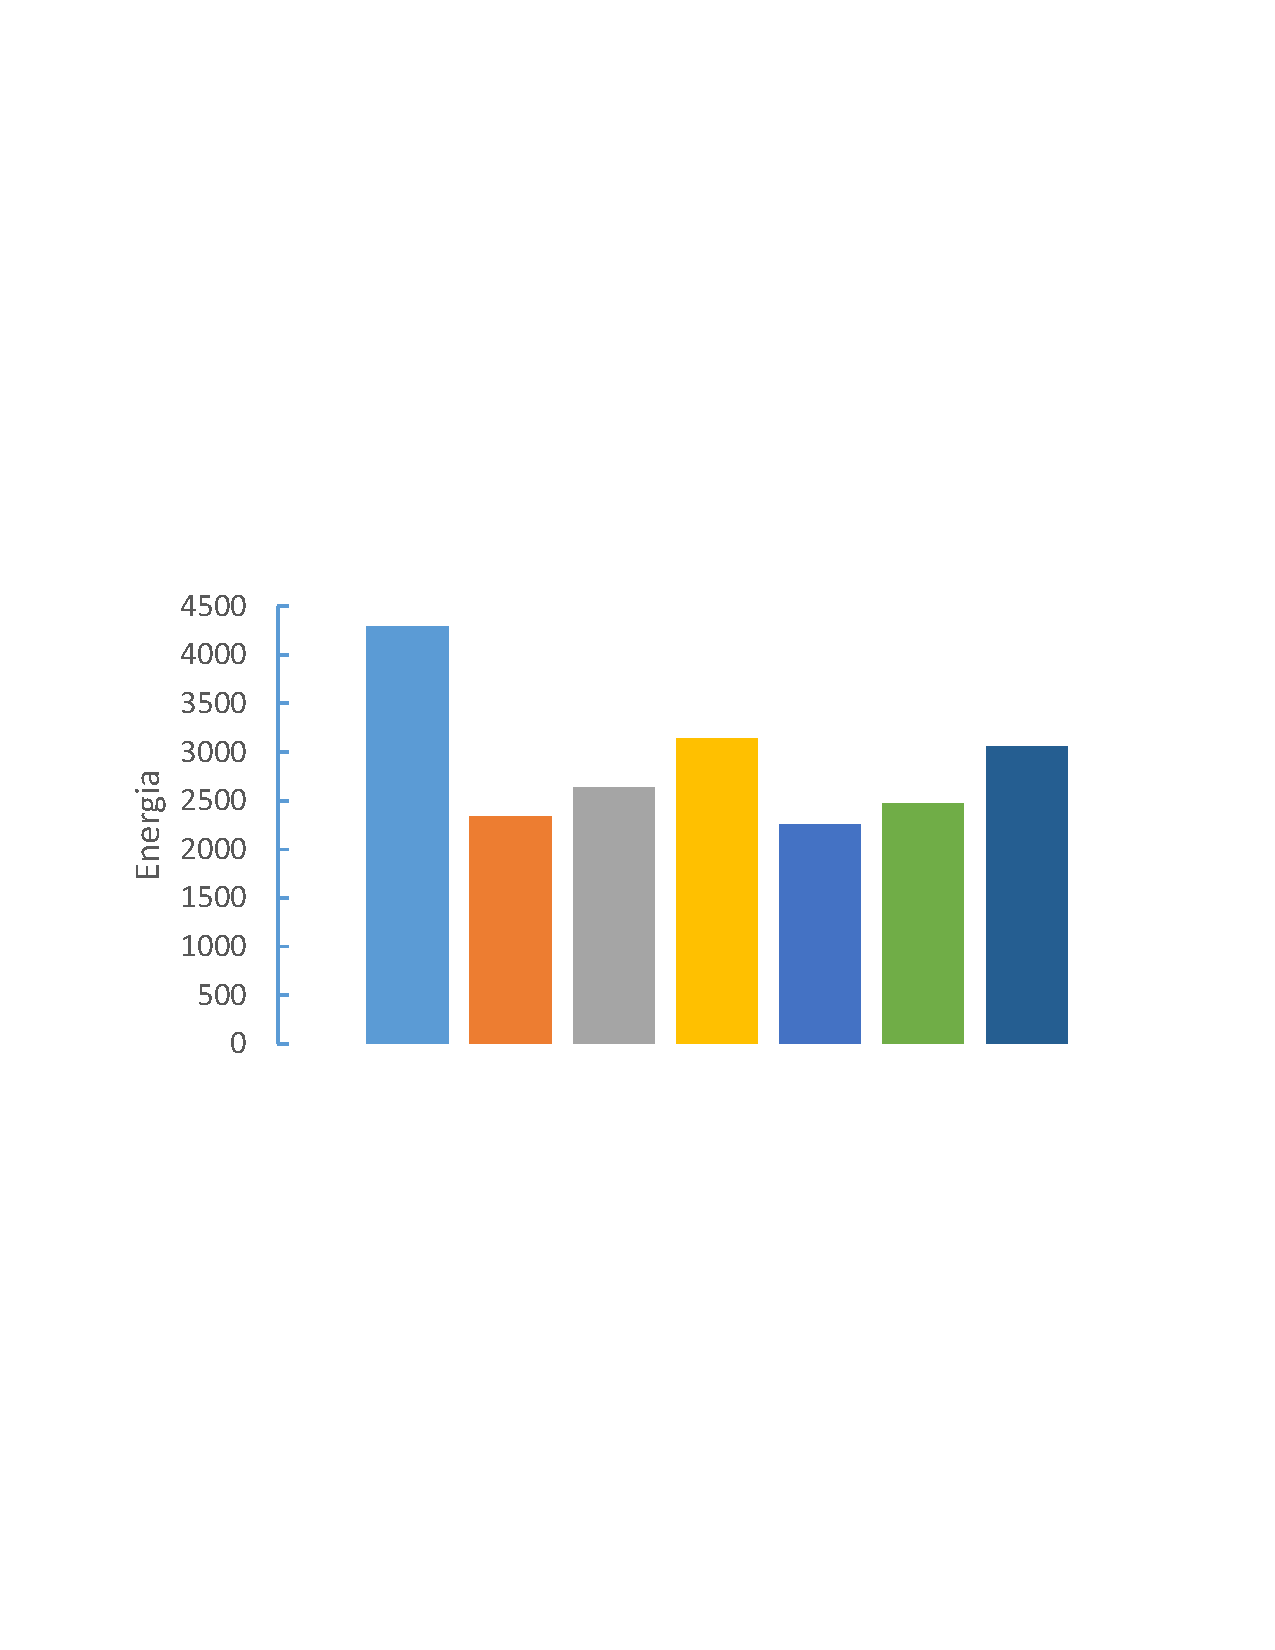
\includegraphics[width= 5cm]{charts/energia_asc.pdf}}\
%\qquad
\subfloat[][]{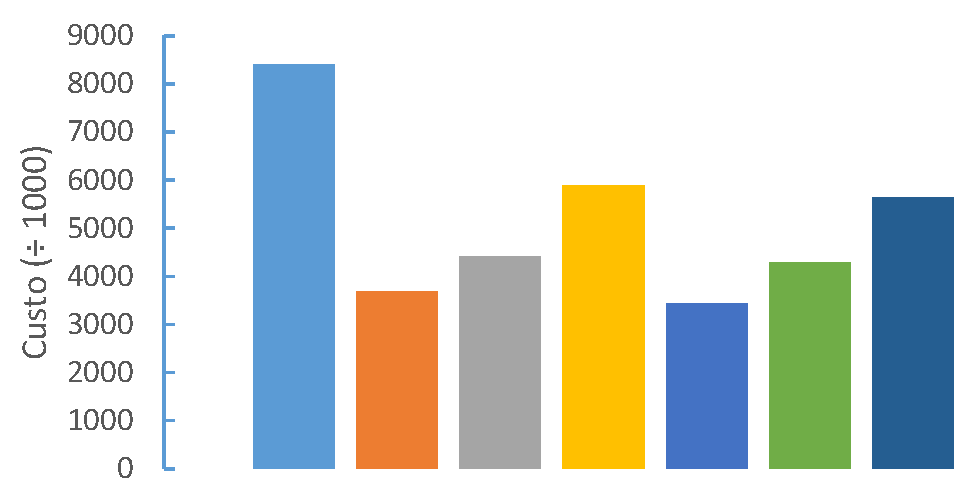
\includegraphics[width= 5cm]{charts/cost_asc.pdf}}\
\end{figure}
\begin{figure}[ht!]
\ContinuedFloat
\caption{Desempenho para aplicação descendente (cont. R. abrevia para contêineres rígidos e cont. F. para contêineres flexíveis para limite de CPU utilizada)}%
\label{fig:perf_des}%
\centering
\vspace{-0.5\baselineskip}
\subfloat[][]{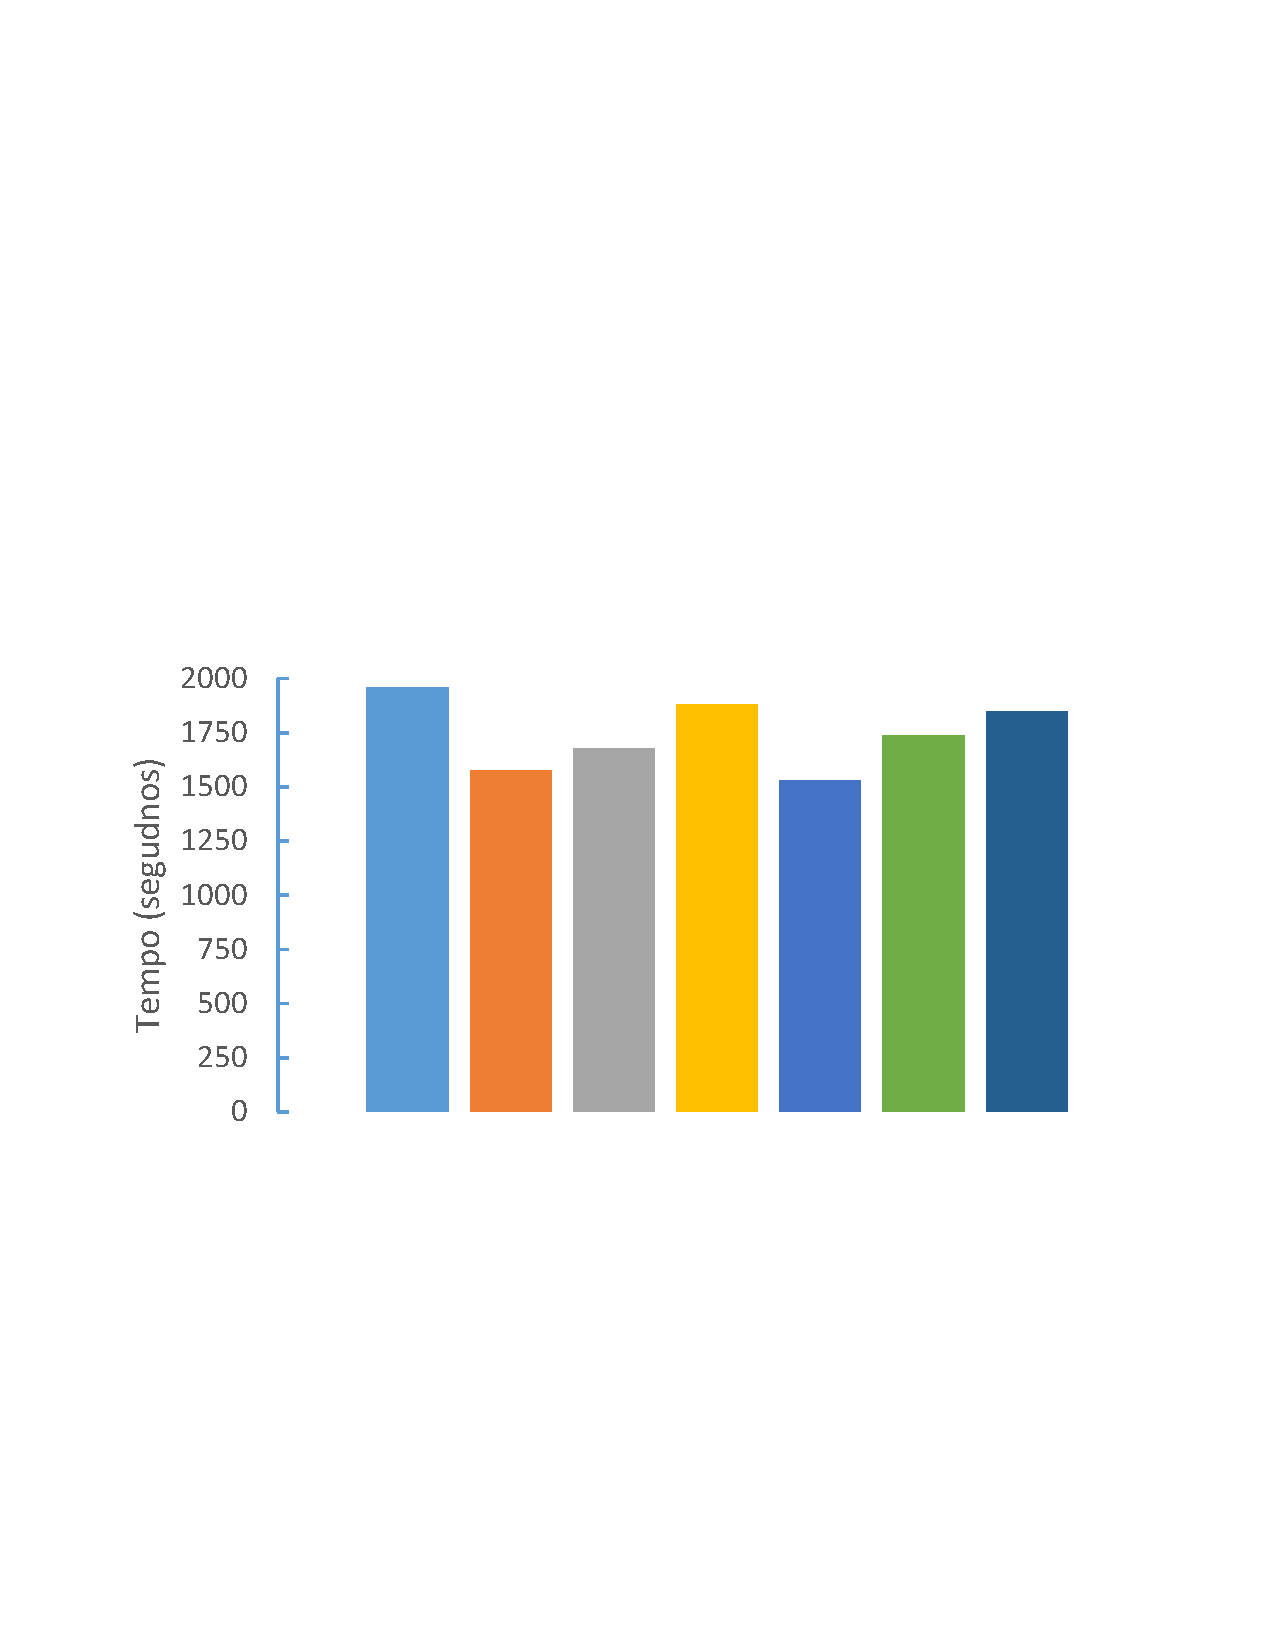
\includegraphics[width= 5cm]{charts/tempo_asc.pdf}}\
%\qquad
\subfloat[][]{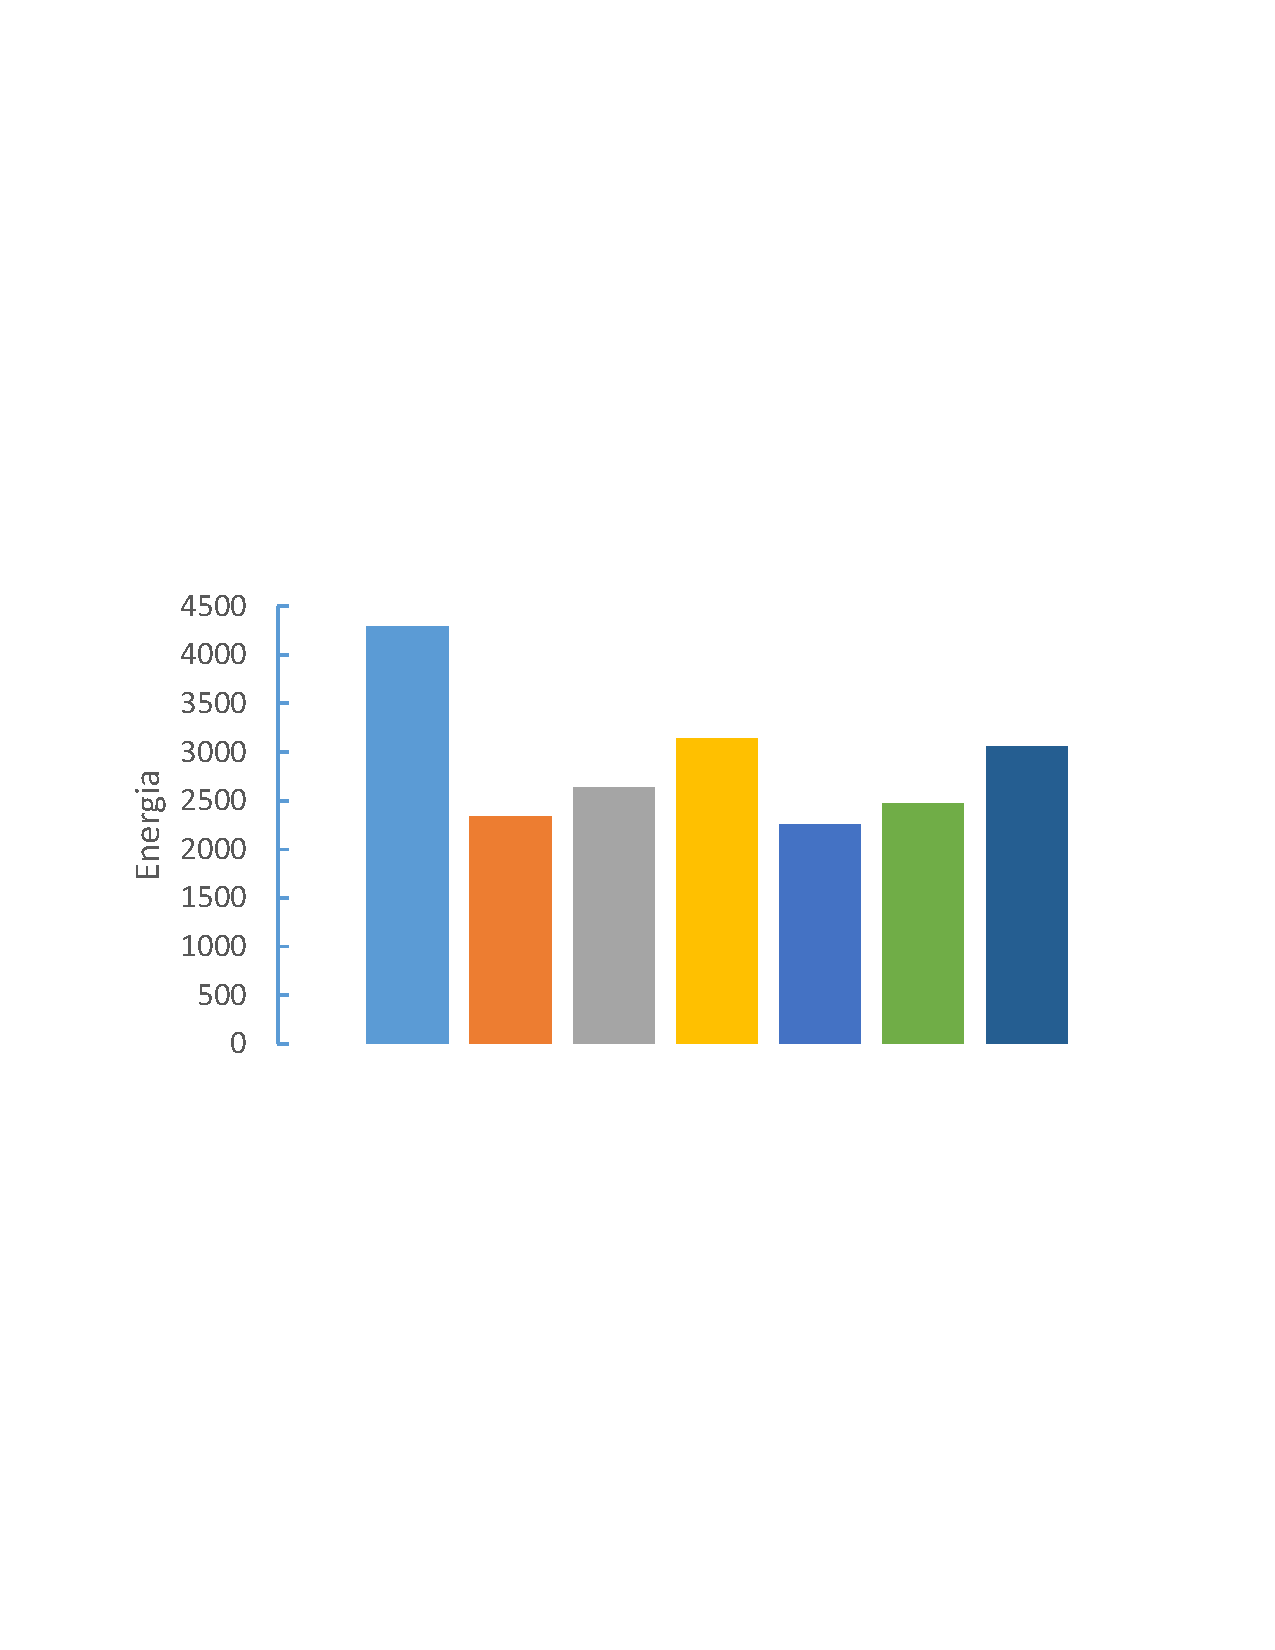
\includegraphics[width= 5cm]{charts/energia_asc.pdf}}\
%\qquad
\subfloat[][]{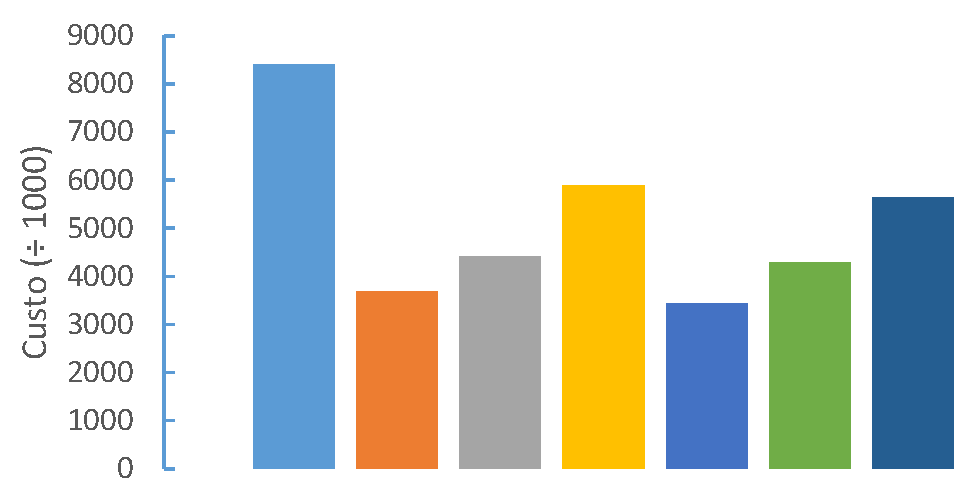
\includegraphics[width= 5cm]{charts/cost_asc.pdf}}\
\end{figure}

\begin{comment}
Colocar um gráfico ilustrando diferença

Comparar especificamente 2 por 2 , fazer uma tabelinha:
Perfil de carga | Virtualização | tempo de alocação | tempo de desalocação | Tempo | Custo
ascending            VM              160                  nao                 
\end{comment}

%=======================================================================
% CONCLUSÃO
%=======================================================================
\section{Conclusão}
\label{conclusion}

Neste trabalho, inicialmente foi realizado uma pesquisa do estado-da-arte de virtualização de recursos para ambientes PAD e \textit{benchmarks} em cima da utilização de contêineres e máquinas virtuais. A partir da pesquisa, foi identificado uma lacuna na literatura quanto à diferença que pode ter ao utilizar uma tecnologia ou outra em ambientes de Nuvem com elasticidade. Com o objetivo de preencher essa lacuna, este artigo propôs o DoCB, um \textit{benchmarking} sobre as estratégias de virtualização e o impacto na Nuvem com elasticidade. O modelo propôe uma série de execuções de uma aplicação em Nuvem com elasticidade, partindo de uma abordagem com máquinas virtuais, para formar a base de comparação, seguindo de execuções variando o número de contêineres por nó, bem como variando também o limite de CPU por contêiner (Rígido e Flexível), um recurso que não existe na virtualização com hipervisores. O diferencial deste \textit{benchmarking} em relação aos outros trabalhos, é a exploração da elasticidade e alocação dinâmica de novos recursos. Outra contribuição foi a análise de desempenho de contêineres variado o número de instâncias por nó e considerando vantagens específicas de contêineres, como o limite de CPU Flexível. 

A fim de executar o \textit{benchmarking} proposto, foi feita uma outra contribuição técnica, que é a adaptação do gerenciador de Nuvem (AutoElastic) para suportar a utilização de contêineres. O gerenciador atuou com os vários cenários de virtualização para uma aplicação com dois tipos de carga: ascendente e descendente. Os resultados foram avaliados segundo as métricas de tempo total de execução, energia e custo (tempo x energia). Nos testes com carga ascendente, a utilização de 2 contêineres por nó com CPU Flexível, apresentou um tempo de aproximadamente 20\% menor que o teste com 2 máquinas virtuais. Ainda, por causa da energia gasta com nós adicionais, a mesma execução com contêineres apresentou um custo de aproximadamente 60\% menor que a execução com máquinas virtuais. 

Como sugestão de trabalhos futuros, indica-se a análise de aplicações variando \textit{thresholds} e explorar outros aspectos de contêineres Docker. Outra possibilidade é a implementação em um ambiente produtivo e verificar o comportamento do gerenciador com as técnicas de virtualização utilizando cargas reais. 

\begin{comment}
- Dados numéricos, números, percentual mais significativo.


A questão de pesquisa original tratava da possibilidade de se otimizar a camada de virtualização de ambientes em nuvem para execução de aplicações HPC, com o objetivo de identificar também as vantagens e situações onde a virtualização por contêineres pode ser uma melhor alternativa. A partir da avaliação dos trabalhos relacionados, foi concluído que em uma comparação 1 pra 1 de máquina virtual e container, a segunda tecnologia se sobressai em questões de desempenho, confirmando, assim, que é possível otimizar o modelo de elasticidade em nuvem ao substituir a camada de virtualização, passando a utilizar contêineres. Sendo assim, decidimos expandir a questão para analisar o desempenho em situações de elasticidade, onde os recursos precisam ser provisionados conforme a demanda, passando a identificar também o que ocorre e o tempo necessário para as etapas de provisionamento. 

Esperamos também que o modelo e resultados da pesquisa possam servir com um guia para outros pesquisadores poderem identificar qual a tecnologia mais adequada para seus objetivos, a partir da verificação de quais parâmetros são necessários. Pois pretendemos identificar, por exemplo, qual solução é mais indicada para aplicações altamente paralelizadas e cenários onde a variação de consumo de recursos pode variar bastante.

Explicar aqui o que pode ter de furo na implementação, o que não deu tempo de fazer etc.
\end{comment}
%=======================================================================
% Abstract IngL~es
%=======================================================================

\begin{otherlanguage}{english}
\othertitle{The Title in English}
\begin{abstract}
Este documento apresenta orientações para uso da classe \LaTeX\ de formatação de artigos para a UNISINOS\@.  Ao mesmo tempo, ele serve como exemplo de uso da classe, demonstrando os principais comandos a serem utilizados, e outras orientações mais gerais de uso do \LaTeX.  Adicionalmente, procuramos incluir no documento algumas orientações sobre a escrita da monografia em si, reunindo dicas e recomendações que contribuem para aumentar a qualidade técnica dos trabalhos acadêmicos.  O Resumo deve conter de 150 a 250~palavras e apresentar o objetivo, o método, os resultados e as conclusões do artigo. Deve ser composto por frases concisas e afirmativas. Recomenda-se o uso de parágrafo único. Deve-se usar o verbo na voz ativa e na terceira pessoa do singular.
\palavraschave{UNISINOS\@.  ABNT\@.  Formatação de documentos.  \LaTeX.}
\end{abstract}
\end{otherlanguage}


%=======================================================================
% Referências
%=======================================================================
\bibliography{exemplo}

%=======================================================================
% Exemplo de Apêndice
% O Apêndice é utilizado para apresentar material complementar elaborado
% pelo próprio autor.  Deve seguir as mesmas regras de formatação do
% corpo principal do documento.
%=======================================================================
%\appendix

%=======================================================================
% Exemplo de Anexo
% O Anexo é utilizado para a ``inclusão de materiais não elaborados pelo
% próprio autor, como cópias de artigos, manuais, folders, balancetes, etc.
% e não precisam estar em conformidade com o modelo''.
%=======================================================================
%\annex

\end{document}
